%%%%%%%%%%%%%%%%%%%%%%%%%%%%%%%%%%%%%%%%%%%%%%%%%%%%%%%%%%%%%%%%%%%%%%%%%%%%%%
%
\chapter{Nonlinear State Space Estimation}
\label{ch:nonlinear-estimation}
%
%%%%%%%%%%%%%%%%%%%%%%%%%%%%%%%%%%%%%%%%%%%%%%%%%%%%%%%%%%%%%%%%%%%%%%%%%%%%%%

In many cases interesting dynamic systems are not linear by nature, so the
traditional Kalman filter cannot be applied in estimating the state of such a
system. In these kind of systems, both the dynamics and the measurement processes
can be nonlinear, or only one them. In this section, we describe two extensions
to the traditional Kalman filter, which can be applied for estimating nonlinear
dynamical systems by forming Gaussian approximations to the joint distribution of
the state $\vec{x}$ and measurement $\vec{y}$. First we present the Extended Kalman
filter (EKF), which is based on Taylor series approximation of the joint
distribution, and then the Unscented Kalman filter (UKF), which is
respectively based on the unscented transformation of the joint distribution.      


%%%%%%%%%%%%%%%%%%%%%%%%%%%%%%%%%%%%%%%%%%%%%%%%%%%%%%%%%%%%%%%%%%%%%%%%%%%%%%
%


\section{Extended Kalman Filter}


\subsection{Taylor Series Based Approximations}

Next we present linear and quadratic approximations for the
distribution of variable $\vec{y}$, which is generated with a non-linear transformation
of a Gaussian random variable $\vec{x}$ as follows:
%
\begin{equation}
\begin{split}
  \vec{x} &\sim \N(\vec{m},\mat{P}) \\
  \vec{y} &= \vec{g}(\vec{x}),
\end{split}
\label{eq:trans_g}
\end{equation}
%
where $\vec{x} \in \spc{R}^n$, $\vec{y} \in \spc{R}^m$, and $\vec{g} :
\spc{R}^n \mapsto \spc{R}^m$ is a general non-linear function. Solving
the distribution of $\vec{y}$ formally is in general not possible,
because it is non-Gaussian for all by linear $\vec{g}$, so in practice
it must be approximated somehow. The joint distribution of $\vec{x}$
and $\vec{y}$ can be formed with, for example, linear and quadratic
approximations, which we present next. See, for example, \citet{Bar-Shalom+Li+Kirubarajan:2001} for the derivation of these approximations.

\subsection{Linear Approximation}

The linear approximation based Gaussian approximation of the joint
distribution of variables $\vec{x}$ and $\vec{y}$ defined by equations
(\ref{eq:trans_g}) is given as
  %
  \begin{equation}
     \begin{pmatrix}
       \vec{x} \\ \vec{y}
     \end{pmatrix} \sim
     \N\left(
     \begin{pmatrix}
       \vec{m} \\ \vecmu_L
     \end{pmatrix},
     \begin{pmatrix}
       \vec{P}   & \vec{C}_L \\
       \vec{C}_L^T & \mat{S}_L
     \end{pmatrix} \right),
  \end{equation}
  %
  where
  %
  \begin{equation}
  \begin{split}
  \vecmu_L &= \vec{g}(\vec{m}) \\
    \mat{S}_L &= \mat{G}_{\vec{x}}(\vec{m}) \, \mat{P} \,
    \mat{G}^T_{\vec{x}}(\vec{m}) \\
    \mat{C}_L &= \mat{P} \, \mat{G}^T_{\vec{x}}(\vec{m}),
  \end{split}
  \end{equation}
  %
  and $\mat{G}_{\vec{x}}(\vec{m})$ is the Jacobian matrix of $\vec{g}$
  with elements
  %
  \begin{equation}
    \left[ \mat{G}_{\vec{x}}(\vec{m}) \right]_{j,j'} =
    \frac{\partial g_j(\vec{x})}{\partial x_{j'}}
    \Bigg|_{\vec{x} = \vec{m}}.
  \label{eq:G1}
  \end{equation}

\subsection{Quadratic Approximation}

The quadratic approximations retain also the second order terms of the
Taylor series expansion of the non-linear function:
  %
  \begin{equation}
     \begin{pmatrix}
       \vec{x} \\ \vec{y}
     \end{pmatrix} \sim
     \N\left(
     \begin{pmatrix}
       \vec{m} \\ \vecmu_Q
     \end{pmatrix},
     \begin{pmatrix}
       \vec{P}   & \vec{C}_Q \\
       \vec{C}_Q^T & \mat{S}_Q
     \end{pmatrix} \right),
  \end{equation}
  %
  where the parameters are
  %
  \begin{equation}
  \begin{split}
  \vecmu_Q &= \vec{g}(\vec{m}) 
  + \frac{1}{2} \sum_i \vec{e}_i \, \tr\left\{
     \mat{G}_{\vec{x}\vec{x}}^{(i)}(\vec{m}) \,
    \mat{P} \right\} \\
    \mat{S}_Q &= \mat{G}_{\vec{x}}(\vec{m}) \, \mat{P} \, \mat{G}^T_{\vec{x}}(\vec{m})
  + \frac{1}{2} \sum_{i,i'} \vec{e}_i \, \vec{e}^T_{i'} \,
    \tr\left\{ \mat{G}_{\vec{x}\vec{x}}^{(i)}(\vec{m}) \, \mat{P} \,
     \mat{G}_{\vec{x}\vec{x}}^{(i')}(\vec{m}) \, \mat{P} \right\} \\
    \mat{C}_Q &= \mat{P} \, \mat{G}^T_{\vec{x}}(\vec{m}),
  \end{split}
  \end{equation}
%
  $\mat{G}_{\vec{x}}(\vec{m})$ is the Jacobian matrix \eqref{eq:G1}
  and $\mat{G}_{\vec{x}\vec{x}}^{(i)}(\vec{m})$ is the Hessian matrix
  of $g_i(\cdot)$ evaluated at $\vec{m}$:
%
\begin{equation}
   \left[ \mat{G}_{\vec{x}\vec{x}}^{(i)}(\vec{m}) \right]_{j,j'}
   = \frac{\partial^2 g_i(\vec{x})}{\partial x_j \, \partial x_{j'}},
  \Bigg|_{\vec{x} = \vec{m}}.
\end{equation}
%
$\vec{e}_i = (0~\cdots~0~1~0~\cdots~0)^T$ is the unit
vector in direction of the coordinate axis $i$.



\subsection{Extended Kalman filter}
%
%%%%%%%%%%%%%%%%%%%%%%%%%%%%%%%%%%%%%%%%%%%%%%%%%%%%%%%%%%%%%%%%%%%%%%%%%%%%%%

The extended Kalman filter \citep[see, for instance, ][]{Jazwinski:1966,
Maybeck:1982,Bar-Shalom+Li+Kirubarajan:2001,Grewal+Andrews:2001,Sarkka:2006} extends the scope of Kalman filter to nonlinear optimal
filtering problems by forming a Gaussian approximation to the joint
distribution of state $\vec{x}$ and measurements $\vec{y}$ using a
Taylor series based transformation. First and second order extended
Kalman filters are presented, which are based on linear and quadratic
approximations to the transformation. Higher order filters are also
possible, but not presented here.


The filtering model used in the EKF is
%
\begin{equation}
\begin{split}
\vec{x}_{k} &= \vec{f}(\vec{x}_{k-1},k-1) + \vec{q}_{k-1} \\
\vec{y}_{k} &= \vec{h}(\vec{x}_{k},k) + \vec{r}_{k},
\end{split} \label {eq:nonlinear_prob}
\end{equation}
%
where $\vec{x}_k \in \spc{R}^n$ is the state, $\vec{y}_k \in
\spc{R}^m$ is the measurement, $\vec{q}_{k-1} \sim
\N(\vec{0},\mat{Q}_{k-1})$ is the process noise, $\vec{r}_{k} \sim
\N(\vec{0},\mat{R}_{k})$ is the measurement noise, $\vec{f}$ is the
(possibly nonlinear) dynamic model function and $\vec{h}$ is the
(again possibly nonlinear) measurement model function. The first and
second order extended Kalman filters approximate the distribution of
state $\vec{x}_k$ given the observations $\vec{y}_{1:k}$ with a
Gaussian:
%
\begin{equation}
  p(\vec{x}_{k}\,|\,\vec{y}_{1:k}) \approx
    \N(\vec{x}_{k}\,|\,\vec{m}_{k},\mat{P}_{k}).
\end{equation}
%

\subsubsection{First Order Extended Kalman Filter}

Like Kalman filter, also the extended Kalman filter is separated to
two steps.  The steps for the first order EKF are as follows:
  %
  \begin{itemize}
  \item {\em Prediction:}
  %
  \begin{equation}
  \begin{split}
    \vec{m}^-_{k} &= \vec{f}(\vec{m}_{k-1},k-1) \\
    \mat{P}^-_{k} &= \mat{F}_{\vec{x}}(\vec{m}_{k-1},k-1) \, \mat{P}_{k-1} \,
     \mat{F}_{\vec{x}}^T (\vec{m}_{k-1},k-1) + \mat{Q}_{k-1}.
  \end{split}
  \label{eq:dekf_predict1}
  \end{equation}
  
  \item {\em Update:}
  %
  \begin{equation}
  \begin{split}
    \vec{v}_{k} &= \vec{y}_k - \mat{h} (\vec{m}^-_{k},k) \\
    \vec{S}_{k} &= \mat{H}_{\vec{x}}(\vec{m}^-_{k},k) \, \mat{P}^-_{k} \,
    \mat{H}^T_{\vec{x}}(\vec{m}^-_{k},k) + \vec{R}_{k} \\
    \vec{K}_{k} &= \mat{P}^-_{k} \, \mat{H}^T_{\vec{x}}(\vec{m}^-_{k},k) \,
    \vec{S}^{-1}_{k} \\
    \vec{m}_{k} &= \vec{m}^-_{k} + \vec{K}_{k} \, \vec{v}_k \\
    \mat{P}_{k} &= \mat{P}^-_{k} - \vec{K}_{k} \, \vec{S}_{k} \, \vec{K}^T_{k},
  \end{split}
  \label{eq:dekf_update1}
  \end{equation}
  \end{itemize}
  %
  where the matrices $\mat{F}_{\vec{x}}(\vec{m},k-1)$ and
  $\mat{H}_{\vec{x}}(\vec{m},k)$ are the Jacobians of
  $\vec{f}$ and $\vec{h}$, with elements
  %
  \begin{align}
    \left[ \mat{F}_{\vec{x}}(\vec{m},k-1) \right]_{j,j'} =
    \frac{\partial f_j(\vec{x},k-1)}{\partial x_{j'}}
    \Bigg|_{\vec{x} = \vec{m}}
  \label{eq:F1} \\
    \left[ \mat{H}_{\vec{x}}(\vec{m},k) \right]_{j,j'} =
    \frac{\partial h_j(\vec{x},k)}{\partial x_{j'}}
    \Bigg|_{\vec{x} = \vec{m}}.
  \label{eq:H1}
  \end{align}
%
Note that the difference between first order EKF and KF is that the
matrices $\mat{A}_k$ and $\mat{H}_k$ in KF are replaced with Jacobian
matrices $\mat{F}_{\vec{x}}(\vec{m}_{k-1},k-1)$ and
$\mat{H}_{\vec{x}}(\vec{m}_k^-,k)$ in EKF. Predicted mean
$\vec{m}_k^-$ and residual of prediction $\vec{v}_k$ are also
calculated differently in the EKF.  In this toolbox the prediction and
update steps of the first order EKF can be computed with functions
\texttt{ekf\_predict1} and \texttt{ekf\_update1}, respectively.

\subsubsection{Second Order Extended Kalman Filter}

The corresponding steps for the second order EKF are as follows:
  %
  \begin{itemize}
  \item {\em Prediction:}
  %
  \begin{equation}
  \begin{split}
    \vec{m}^-_{k} &= \vec{f}(\vec{m}_{k-1},k-1) 
    + \frac{1}{2} \sum_i \vec{e}_i \,
      \tr\left\{ \mat{F}_{\vec{x}\vec{x}}^{(i)}(\vec{m}_{k-1},k-1) \,
      \mat{P}_{k-1} \right\} \\
    \mat{P}^-_{k} &= \mat{F}_{\vec{x}}(\vec{m}_{k-1},k-1) \, \mat{P}_{k-1} \,
     \mat{F}^T_{\vec{x}}(\vec{m}_{k-1},k-1) \\
   &+ \frac{1}{2} \sum_{i,i'} \vec{e}_i \, \vec{e}^T_{i'}
      \tr\left\{ \mat{F}_{\vec{x}\vec{x}}^{(i)}(\vec{m}_{k-1},k-1) \mat{P}_{k-1} 
       \mat{F}_{\vec{x}\vec{x}}^{(i')}(\vec{m}_{k-1},k-1) \mat{P}_{k-1} \right\} \\
    &+ \mat{Q}_{k-1}.
  \end{split}
  \label{eq:dekf_predict2}
  \end{equation}

  \item {\em Update:}
  %
  \begin{equation}
  \begin{split}
    \vec{v}_{k} &= \vec{y}_k - \mat{h} (\vec{m}^-_{k},k) 
    - \frac{1}{2} \sum_i \vec{e}_i \,
      \tr\left\{ \mat{H}_{\vec{x}\vec{x}}^{(i)}(\vec{m}^-_{k},k) \,
      \mat{P}^-_{k} \right\} \\
    \vec{S}_{k} &= \mat{H}_{\vec{x}}(\vec{m}^-_{k},k) \, \mat{P}^-_{k} \,
    \mat{H}^T_{\vec{x}}(\vec{m}^-_{k},k) \\
    &\quad + \frac{1}{2} \sum_{i,i'} \vec{e}_i \, \vec{e}^T_{i'} \,
      \tr\left\{ \mat{H}_{\vec{x}\vec{x}}^{(i)}(\vec{m}^-_{k},k) \, \mat{P}^-_{k} \,
       \mat{H}_{\vec{x}\vec{x}}^{(i')}(\vec{m}^-_{k},k) \, \mat{P}^-_{k} \right\} 
    + \vec{R}_{k} \\
    \vec{K}_{k} &= \mat{P}^-_{k} \,
    \mat{H}^T_{\vec{x}}(\vec{m}^-_{k},k) \, \vec{S}^{-1}_{k} \\
    \vec{m}_{k} &= \vec{m}^-_{k} + \vec{K}_{k} \, \vec{v}_k \\
    \mat{P}_{k} &= \mat{P}^-_{k} - \vec{K}_{k} \, \vec{S}_{k} \, \vec{K}^T_{k},
  \end{split}
  \label{eq:dekf_update2}
  \end{equation}
  \end{itemize}
  %
  where matrices $\mat{F}_{\vec{x}}(\vec{m},k-1)$ and
  $\mat{H}_{\vec{x}}(\vec{m},k)$ are Jacobians as in the first order EKF, given by
  Equations \eqref{eq:F1} and \eqref{eq:H1}. The matrices
  $\mat{F}^{(i)}_{\vec{x}\vec{x}}(\vec{m},k-1)$ and
  $\mat{H}^{(i)}_{\vec{x}\vec{x}}(\vec{m},k)$ are the Hessian matrices
  of $f_i$ and $h_i$:
  \begin{align}
   \left[ \mat{F}_{\vec{x}\vec{x}}^{(i)}(\vec{m},k-1) \right]_{j,j'}
   = \frac{\partial^2 f_i(\vec{x},k-1)}{\partial x_j \, \partial x_{j'}}
  \Bigg|_{\vec{x} = \vec{m}}
  \label{eq:F2} \\
   \left[ \mat{H}_{\vec{x}\vec{x}}^{(i)}(\vec{m},k) \right]_{j,j'}
   = \frac{\partial^2 h_i(\vec{x},k)}{\partial x_j \, \partial x_{j'}}
  \Bigg|_{\vec{x} = \vec{m}},
  \label{eq:H2}
  \end{align}
%
$\vec{e}_i = (0~\cdots~0~1~0~\cdots~0)^T$ is a unit vector in direction of the
coordinate axis $i$, that is, it has a $1$ at position $i$ and $0$ at other positions.

The prediction and update steps of the second order EKF can be
computed in this toolbox with functions \texttt{ekf\_predict2} and
\texttt{ekf\_update2}, respectively. By taking the second order terms
into account, however, doesn't quarantee, that the results get any
better. Depending on problem they might even get worse, as we shall
see in the later examples.

\subsection{The Limitations of EKF}

As discussed in, for example, \citep{Julier+Uhlmann:2004} the EKF has a
few serious drawbacks, which should be kept in mind when it's used:
%
\begin{enumerate}
\item As we shall see in some of the later demonstrations, the linear
  and quadratic transformations produces realiable results only when
  the error propagation can be well approximated by a linear or a
  quadratic function. If this condition is not met, the performance of
  the filter can be extremely poor. At worst, its estimates can
  diverge altogether.
\item The Jacobian matrices (and Hessian matrices with second order
  filters) need to exist so that the transformation can be applied.
  However, there are cases, where this isn't true. For example, the
  system might be jump-linear, in which the parameters can change
  abruptly \citep{Julier+Uhlmann:2004}.
\item In many cases the calculation of Jacobian and Hessian matrices
  can be a very difficult process, and its also prone to human errors
  (both derivation and programming). These errors are usually very
  hard to debug, as its hard to see which parts of the system produces
  the errors by looking at the estimates, especially as usually we
  don't know which kind of performance we should expect. For example,
  in the last demonstration (Reentry Vehicle Tracking) the first order
  derivatives were quite troublesome to calcute, even though the
  equations themselves were relatively simple. The second order
  derivatives would have even taken many more times of work.
\end{enumerate}
%
\label{page:ekf_problems}


  

%%%%%%%%%%%%%%%%%%%%%%%%%%%%%%%%%%%%%%%%%%%%%%%%%%%%%%%%%%%%%%%%%%%%%%%%%%%%%%
%
\subsection{Extended Kalman smoother}
%
%%%%%%%%%%%%%%%%%%%%%%%%%%%%%%%%%%%%%%%%%%%%%%%%%%%%%%%%%%%%%%%%%%%%%%%%%%%%%%

The difference between the first order extended Kalman smoother \citep{Cox:1964,Sage+Melsa:1971} and the traditional Kalman smoother is the
same as the difference between first order EKF and KF, that is, matrix
$\mat{A}_k$ in Kalman smoother is replaced with Jacobian
$\mat{F}_{\vec{x}}(\vec{m}_{k-1},k-1)$, and $\vec{m}_{k+1}^-$ is
calculated using the model function $\vec{f}$.  Thus, the equations
for the extended Kalman smoother can be written as
%
\begin{equation}
\begin{split}
    \vec{m}^-_{k+1} &= \vec{f}(\vec{m}_{k},k) \\
    \mat{P}^-_{k+1} &= \mat{F}_{\vec{x}}(\vec{m}_{k},k) \, \mat{P}_{k} \,
     \mat{F}_{\vec{x}}^T(\vec{m}_{k},k) + \mat{Q}_{k} \\
    \vec{C}_{k} &= \mat{P}_k \, \mat{F}_{\vec{x}}^T(\vec{m}_{k},k) \,
      [\mat{P}^-_{k+1}]^{-1} \\
    \vec{m}^s_k &= \vec{m}_k
    + \mat{C}_k \, [\vec{m}^s_{k+1} - \vec{m}^-_{k+1}] \\
    \mat{P}^s_k &= \mat{P}_k
    + \mat{C}_k \, [\mat{P}^s_{k+1} - \mat{P}^-_{k+1}] \, \mat{C}^T_k.
    \label{eq:derts}
\end{split}
\end{equation}
%
First order smoothing solutiong with a RTS type smoother can be
computed with function \texttt{erts\_smooth1}, and with
forward-backward type smoother the computation can be done with
function \texttt{etf\_smooth1}.

Higher order smoothers are also possible, but not described here, as
they are not currently implemented in this toolbox.

%%%%%%%%%%%%%%%%%%%%%%%%%%%%%%%%%%%%%%%%%%%%%%%%%%%%%%%%%%%%%%%%%%%%%%%%%%%%%%
%
\section{Demonstration: Tracking a random sine signal}
%
%%%%%%%%%%%%%%%%%%%%%%%%%%%%%%%%%%%%%%%%%%%%%%%%%%%%%%%%%%%%%%%%%%%%%%%%%%%%%%
Next we consider a simple, yet practical, example of a nonlinear
dynamic system, in which we estimate a random sine signal using the
extended Kalman filter. By random we mean that the angular velocity
and the amplitude of the signal can vary through time. In this example
the nonlinearity in the system is expressed through the measurement
model, but it would also be possible to express it with the dynamic
model and let the measurement model be linear.

The state vector in this case can be expressed as
%
\begin{equation}
%
\vec{x}_k = 
\begin{pmatrix}
\theta_k & \omega_k & a_k
\end{pmatrix}^T,
%
\end{equation}
%
where $\theta_k$ is the parameter for the sine function on time step
$k$, $\omega_k$ is the angular velocity on time step $k$ and $a_k$ is
the amplitude on time step $k$. The evolution of parameter $\theta$ is
modelled with a discretized Wiener velocity model, where the velocity
is now the angular velocity:
%
\begin{equation}
%
\frac{d \theta}{d t} = \omega.
%
\end{equation}
%
The values of $\omega$ and $a$ are perturbed with one dimensional
white noise processes $w_a(t)$ and $w_w(t)$, so the signal isn't
totally deterministic:
%
\begin{eqnarray}
%
\frac{da}{dt} &=& w_a(t) \\ \frac{dw}{dt} &=& w_w(t).
%
\end{eqnarray}
%
Thus, the continous-time dynamic equation can be written as
%
\begin{equation}
%
\frac{d \vec{x}(t)}{dt} = \begin{pmatrix} 0 & 1 & 0\\ 0 & 0 & 0\\ 0 &
0 & 0
\end{pmatrix}\vec{x}(t) +
\begin{pmatrix} 0 & 0 \\ 1 & 0 \\ 0 & 1
\end{pmatrix}\vec{w}(t), \label{eq:sine_cont_model}
%
\end{equation}
%
where the white noise process $\vec{w}(t)$ has power spectral density
%
\begin{equation}
%
\mat{Q}_c = \begin{pmatrix} q_1 & 0 \\ 0 & q_2
\end{pmatrix}.
%
\end{equation}
%
Variables $q_1$ and $q_2$ describe the strengths of random
perturbations of the angular velocity and the amplitude, respectively,
which are in this demonstration are set to $q_1 = 0.2$ and $q_2 =
0.1$. By using the equation (\ref{eq:ode_ak}) the discretized form of
the dynamic equation can written as
%
\begin{equation}
%
\vec{x}_k = \begin{pmatrix} 1 & \dt & 0\\ 0 & 1 & 0\\ 0 & 0 & 1
\end{pmatrix}\vec{x}_{k-1} + \vec{q}_{k-1},
%
\end{equation}
%
where $\dt$ is the step size (with value $\dt = 0.01$ in this case),
and using the equation (\ref{eq:ode_qk}) the covariance matrix
$\mat{Q}_{k-1}$ of the discrete Gaussian white noise process
$\vec{q}_{k-1} \sim N(\vec{0},\mat{Q}_{k-1})$ can be easily computed
to give
%
\begin{equation}
%
\mat{Q}_{k-1} = \begin{pmatrix} \frac{1}{3}\dt^3q_1 &
\frac{1}{2}\dt^2q_1 & 0\\ \frac{1}{2}\dt^2q_1 & \dt q_1 & 0\\ 0 & 0 &
\dt q_2
\end{pmatrix}.
\end{equation}
%

As stated above, the non-linearity in this case is expressed by the
measurement model, that is, we propagate the current state through a
non-linear measurement function $\vec{h}(\vec{x}_{k},k)$ to get an
actual measurement. Naturally the function in this case is the actual
sine function
%
\begin{equation}
%
\vec{h}(\vec{x}_{k},k) = a_k\sin(\theta_k). \label{eq:ekf_demo1_h}
%
\end{equation}
%
With this the measurement model can be written as
%
\begin{equation}
%
y_k = \vec{h}(\vec{x}_k,k) + r_k = a_k\sin(\theta_k) + r_k,
%
\end{equation}
%
where $r_k$ is white, univariate Gaussian noise with zero mean and
variance $\sigma_r = 1$.
 
The derivatives of the measurement function with respect to state
variables are
%
\begin{equation}
\begin{split}
%
\frac{\partial \vec{h}(\vec{x}_{k},k)}{\partial \theta_k} &=
a_k\cos(\theta_k)\\ \frac{\partial \vec{h}(\vec{x}_{k},k)}{\partial
\omega_k} &= 0\\ \frac{\partial \vec{h}(\vec{x}_{k},k)}{\partial a_k}
&= \sin(\theta_k),
%
\end{split}
\end{equation}
%
so the Jacobian matrix (actually in this case, a vector, as the
measurements are only one dimensional) needed by the EKF can be
written as
%
\begin{equation}
%
\mat{H}_{\vec{x}}(\vec{m},k) = \begin{pmatrix} a_k\cos(\theta_k) & 0 &
\sin(\theta_k) \label{eq:ekf_demo1_jacobian}
\end{pmatrix}.
%
\end{equation}
%

We also filter the signal with second order EKF, so we need to
evaluate the Hessian matrix of the measurement model function.  In
this case the second order derivatives of $\vec{h}$ with respect to
all state variables can written as

\begin{equation}
\begin{split}
%
\frac{\partial^2 \vec{h}(\vec{x}_{k},k)}{\partial \theta_k \partial
\theta_k} &= -a_k\sin(\theta_k)\\ \frac{\partial^2
\vec{h}(\vec{x}_{k},k)}{\partial \theta_k \partial \omega_k} &= 0\\
\frac{\partial^2 \vec{h}(\vec{x}_{k},k)}{\partial \theta_k \partial
a_k} &= \cos(\theta_k)\\ \frac{\partial^2
\vec{h}(\vec{x}_{k},k)}{\partial \omega_k \partial \omega_k} &= 0\\
\frac{\partial^2 \vec{h}(\vec{x}_{k},k)}{\partial \omega_k \partial
a_k} &= 0\\ \frac{\partial^2 \vec{h}(\vec{x}_{k},k)}{\partial a_k
\partial a_k} &= 0.
%
\end{split}
\end{equation} With these the Hessian matrix can expressed as
%
\begin{equation}
%
\mat{H}_{\vec{xx}}(\vec{m},k) = \begin{pmatrix} -a_k\sin(\theta_k) & 0
& \cos(\theta_k) \\ 0 & 0 & 0 \\ \cos(\theta_k) & 0 & 0
\label{eq:ekf_demo1_hessian}
\end{pmatrix}.
%
\end{equation}
%
Note that as the measurements are only one dimensional we need to
evaluate only one Hessian, and as the expressions are rather simple
the computation of this Hessian is trivial. In case of higher
dimensions we would need to evaluate the Hessian for each dimension
separately, which could easily result in high amount of dense algebra.


In this demonstration program the measurement function
(\ref{eq:ekf_demo1_h}) is computed with the following code:
%
\begin{lstlisting} 
function Y = ekf_demo1_h(x,param) 
  f = x(1,:); 
  a = x(3,:); 
  Y = a.*sin(f); 
  if size(x,1) == 7 Y = Y + x(7,:); end
\end{lstlisting}
%
where the parameter \texttt{x} is a vector containing a single state
value, or a matrix containing multiple state values. It is also
necessary to include the parameter \texttt{param}, which contains the
other possible parameters for the functions (not present in this
case). The last three lines are included for the augmented version of
unscented Kalman filter (UKF), which is described later in this
document.  The Jacobian matrix of the measurement function (eq.
(\ref{eq:ekf_demo1_jacobian})) is computed with the following
function:
%
\begin{lstlisting} 
function dY = ekf_demo1_dh_dx(x, param) 
  f = x(1,:); 
  w = x(2,:); 
  a = x(3,:); 
  dY = [(a.*cos(f))' zeros(size(f,2),1) (sin(f))'];
\end{lstlisting}
%
The Hessian matrix of the measurement function (eq.
\ref{eq:ekf_demo1_hessian}) is computed with the following function:
%
\begin{lstlisting} 
function df = ekf_sine_d2h_dx2(x,param) 
  f = x(1); 
  a = x(3);
  df = zeros(1,3,3); 
  df(1,:,:) = [-a*sin(f) 0 cos(f); 0 0 0; cos(f) 0 0];
\end{lstlisting}
% 
These functions are defined in files \texttt{efk\_sine\_h.m},
\texttt{ekf\_sine\_dh\_dx.m} and \texttt{ekf\_sine\_d2h\_dx2.m},
respectively. The handles of these functions are saved in the actual
demonstration script file (\texttt{ekf\_sine\_demo.m}) with the
following code lines:
%
\begin{lstlisting} 
h_func = @ekf_sine_h; 
dh_dx_func = @ekf_sine_dh_dx;
d2h_dx2_func = @ekf_sine_d2h_dx2;
\end{lstlisting}
%

It is also important to check out that the implementation on
calculating the derivatives is done right, as it is, especially with
more complex models, easy to make errors in the equations. This can be
done with function \texttt{der\_check}:
%
\begin{lstlisting} 
der_check(h_func, dh_dx_func, 1, [f w a]');
\end{lstlisting}
%
The third parameter with value \texttt{1} signals that we want to test
the derivative of function's first (and in this case the only)
dimension.  Above we have assumed, that the variable \texttt{f}
contains the parameter value for the sine function, \texttt{w} the
angular velocity of the signal and \texttt{a} the amplitude of the
signal.

After we have discretized the dynamic model and generated the real
states and measurements same as in the previous example (the actual
code lines are not stated here, see the full source code at end of
this document), we can use the EKF to get the filtered estimates for
the state means and covariances. The filtering (with first order EKF)
is done almost the same as in the previous example:
%
\begin{lstlisting} 
MM = zeros(size(M,1),size(Y,2)); PP =
zeros(size(M,1),size(M,1),size(Y,2));

for k=1:size(Y,2) 
  [M,P] = ekf_predict1(M,P,A,Q); 
  [M,P] = ekf_update1(M,P,Y(:,k),dh_dx_func,R*eye(1),h_func); 
  MM(:,k) = M;
  PP(:,:,k) = P; 
end
\end{lstlisting}
%
As the model dynamics are in this case linear the prediction step
functions exactly the same as in the case of traditional Kalman
filter. In update step we pass the handles to the measurement model
function and it's derivative function and the variance of measurement
noise (parameters 6, 4 and 5, respectively), in addition to other
parameters. These functions also have additional parameters, which
might be needed in some cases. For example, the dynamic and
measurement model functions might have parameters, which are needed
when those functions are called. See the full function specifications
in chapter~\ref{ch:functions} for more details about the parameters.

With second order EKF the filtering loop remains almost the same with
the exception of update step:
%
\begin{lstlisting} 
MM2 = zeros(size(M,1),size(Y,2)); 
PP2 = zeros(size(M,1),size(M,1),size(Y,2));

for k=1:size(Y,2) 
  [M,P] = ekf_predict1(M,P,A,Q); 
  [M,P] = ekf_update2(M,P,Y(:,k),dh_dx_func,...  
    d2h_dx2_func,R*eye(1),h_func);
  MM(:,k) = M; PP(:,:,k) = P; 
end
\end{lstlisting}
%


The smoothing of state estimates using the extended RTS smoother is
done sameways as in the previous example:
%
\begin{lstlisting} 
[SM1,SP1] = erts_smooth1(MM,PP,A,Q);
\end{lstlisting}
%
With the extended forward-backward smoother the smoothing is done with
the following function call:
%
\begin{lstlisting} 
[SM2,SP2] = etf_smooth1(MM,PP,Y,A,Q,[],[],[],...
  dh_dx_func,R*eye(1),h_func);
\end{lstlisting}
%
Here we have assigned empty vectors for parameters 6,7 and 8 (inverse
prediction, its derivative w.r.t. to noise and its parameters,
respectively), because they are not needed in this case.

To visualize the filtered and smoothed signal estimates we must
evaluate the measurement model function with every state estimate to
project the estimates to the measurement space. This can be done with
the built-in Matlab function \texttt{feval}:
%
\begin{lstlisting} 
Y_m = feval(h_func, MM);
\end{lstlisting}
%
The filtered and smoothed estimates of the signals using the first
order EKF, ERTS and ETF are plotted in figures \ref{fig:example2_1},
\ref{fig:example2_2} and \ref{fig:example2_3}, respectively. The
estimates produced by second order EKF are not plotted as they do not
differ much from first order ones.  As can be seen from the figures
both smoothers give clearly better estimates than the
filter. Especially in the beginning of the signal it takes a while for
the filter to catch on to right track.


\label{page:sine_rmse}

The difference between the smoothers doesn't become clear just by
looking these figures. In some cases the forward-backward smoother
gives a little better estimates, but it tends to be more sensitive
about numerical accuracy and the process and measurement noises. To
make a comparison between the performances of different methods we
have listed the average of root mean square errors (RMSE) on 100 Monte
Carlo simulations with different methods in table
\ref{table:sine_errors}.  In addition to RMSE of each state variable
we also provide the estimation error in measurement space, because we
might be more interested in estimating the actual value of signal than
its components.  Usually, however, the primary goal of these methods
is to estimate the hidden state variables. The following methods were
used:
%
\begin{itemize}
\item EKF1: First order extended Kalman filter.
\item ERTS1: First order extended Rauch-Tung-Striebel smoother.
\item ETF1: First order extended Forward-Backward smoother.
\item EKF2: Second order extended Kalman filter.
\item ERTS2: First order extended Rauch-Tung-Striebel smoother applied
to second order EKF estimates.
\item ETF2: First order extended Forward-Backward smoother applied to
second order EKF estimates.
\item UKF: unscented Kalman filter.
\item URTS: unscented Rauch-Tung-Striebel smoother.
\end{itemize}
%
From the errors we can see that with filters EKF2 gives clearly the
lowest errors with variables $\theta$ and $a$. Due to this also with
smoothers ERTS2 and ETF2 give clearly lower errors than others. On the
other hand EKF1 gives the lowest estimation error with variable
$\omega$. Furthermore, with filters EKF1 also gives lowest error in
measurement space. Each smoother, however, gives approximately the
same error in measurement space. It can also be seen, that the UKF
functions the worst in this case. This is due to linear and quadratic
approximations used in EKF working well with this model. However, with
more nonlinear models UKF is often superior over EKF, as we shall see
in later sections.

In all, none of the used methods proved to be clearly superior over
the others with this model. It is clear, however, that EKF should be
preferred over UKF as it gives lower error and is slightly less
demanding in terms of computation power.  Whether first or second
order EKF should be used is ultimately up to the goal of
application. If the actual signal value is of interest, which is
usually the case, then one should use first order EKF, but second
order one might better at predicting new signal values as the
variables $\theta$ and $a$ are closer to real ones on average.

\begin{figure}
\begin{center}
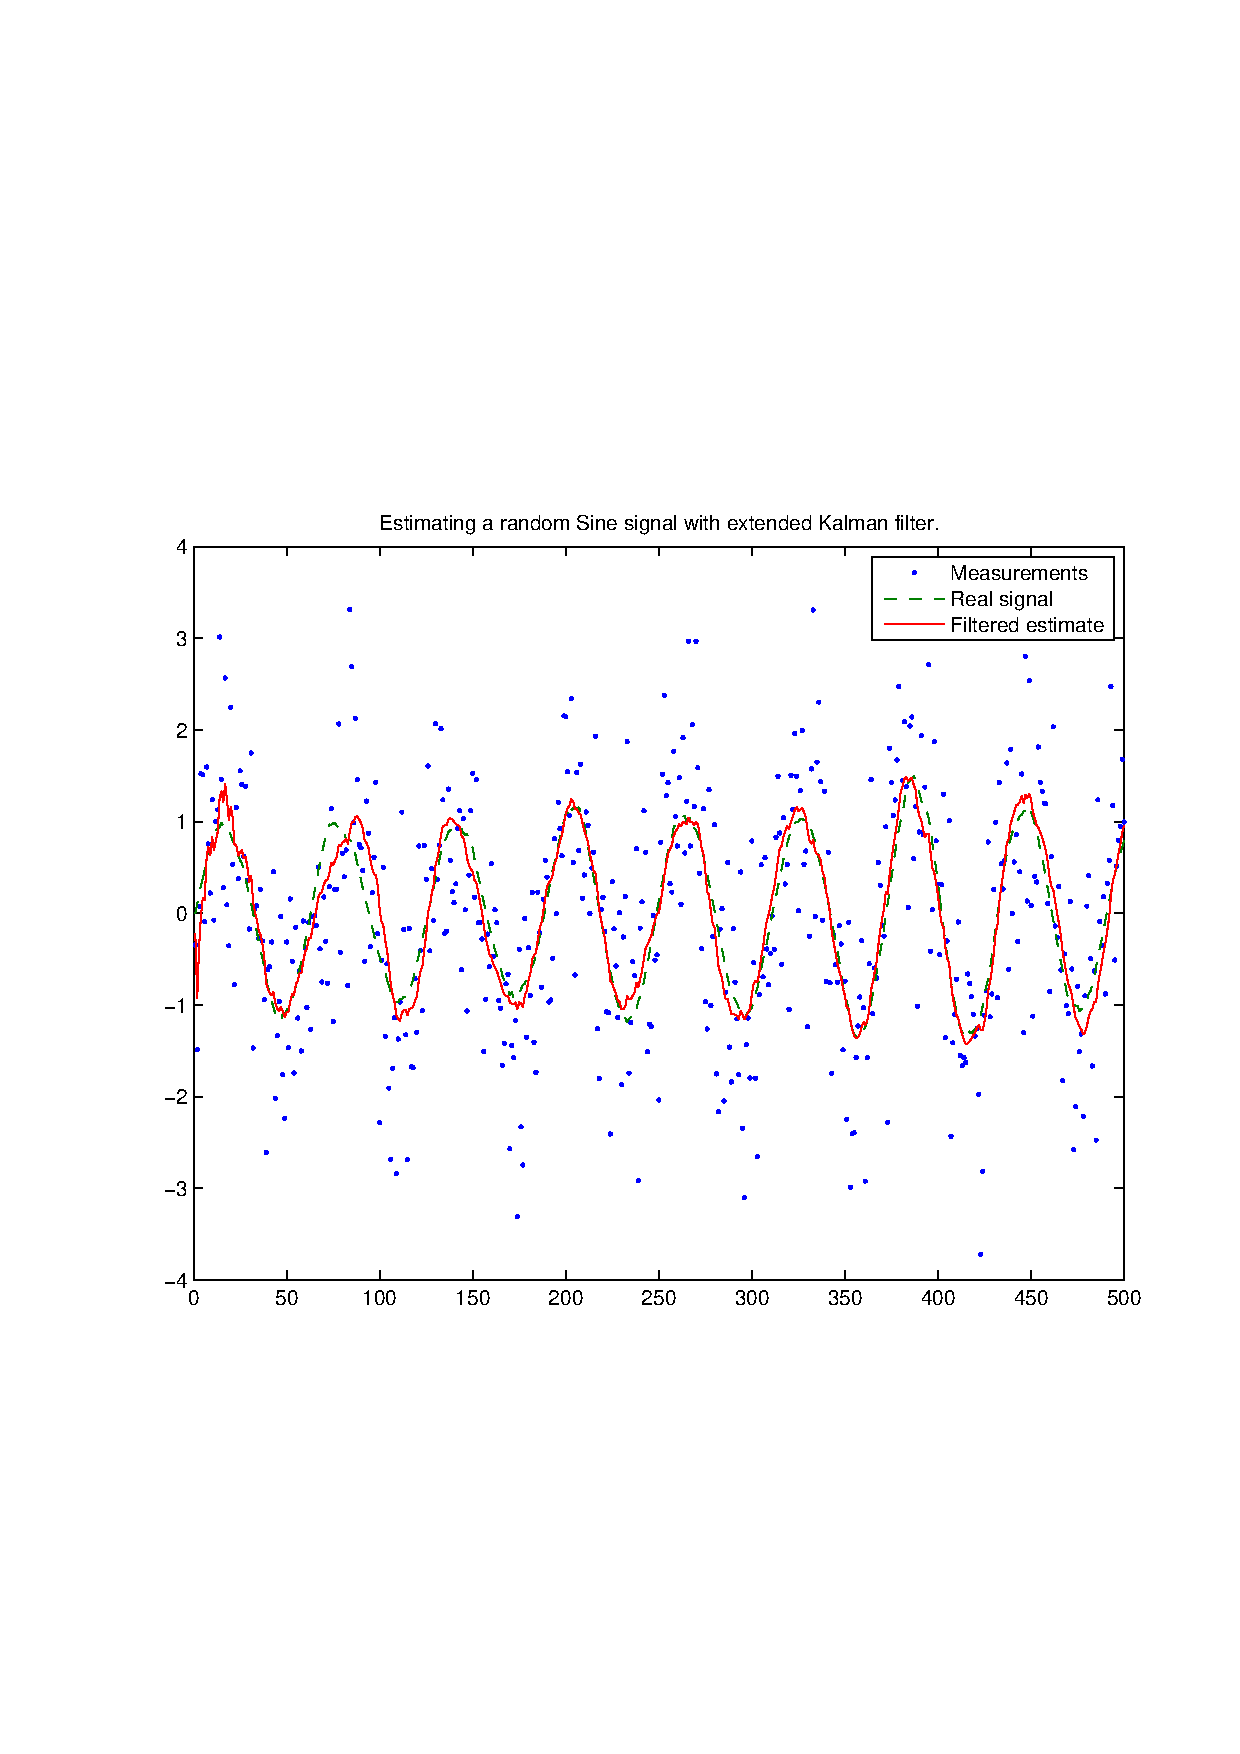
\includegraphics[width=11cm]{pics/demo2_f1}
\caption{Filtered estimate of the sine signal using the first order
extended Kalman filter.}
\label{fig:example2_1}
\end{center}
\end{figure}

\begin{figure}
\begin{center}
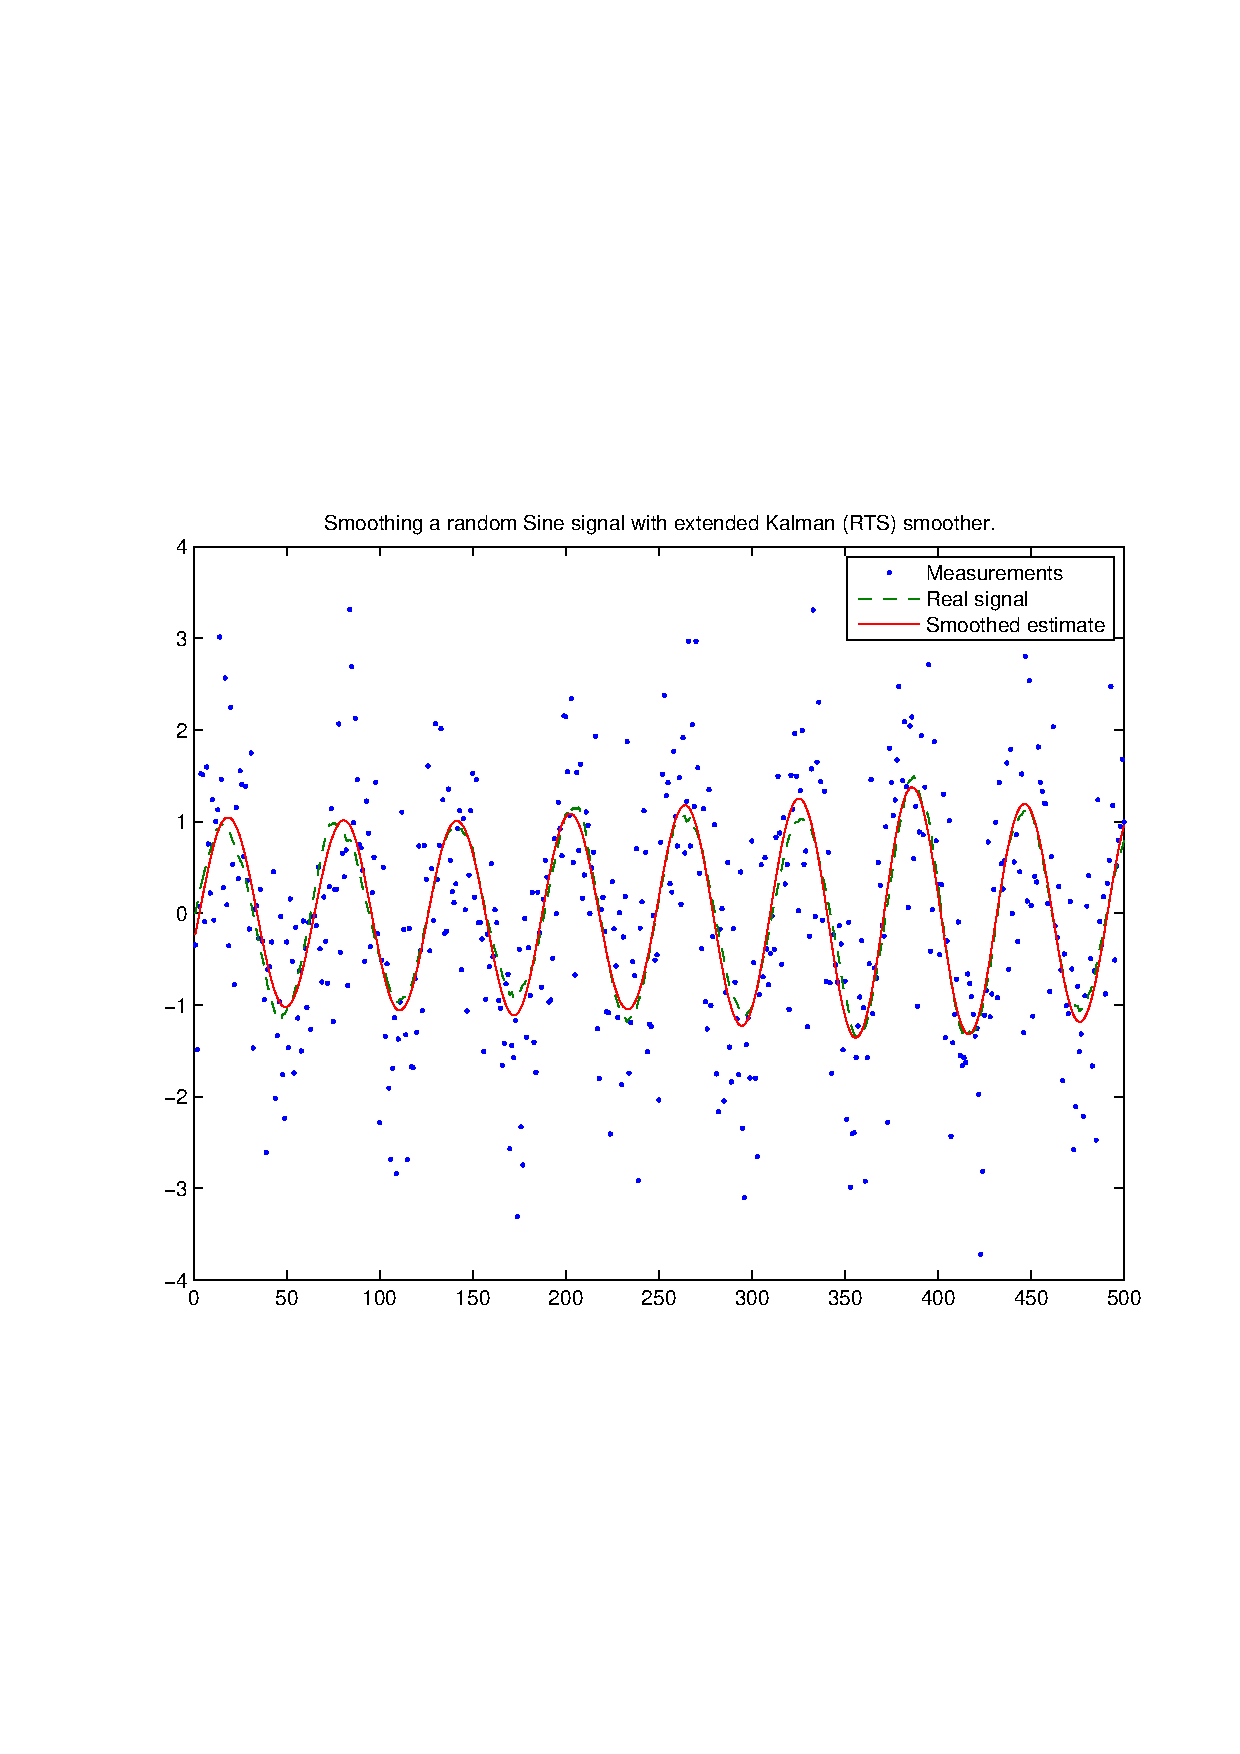
\includegraphics[width=11cm]{pics/demo2_f2}
\caption{Smoothed estimate of the sine signal using the extended
Kalman (RTS) smoother.}
\label{fig:example2_2}
\end{center}
\end{figure}

\begin{figure}
\begin{center}
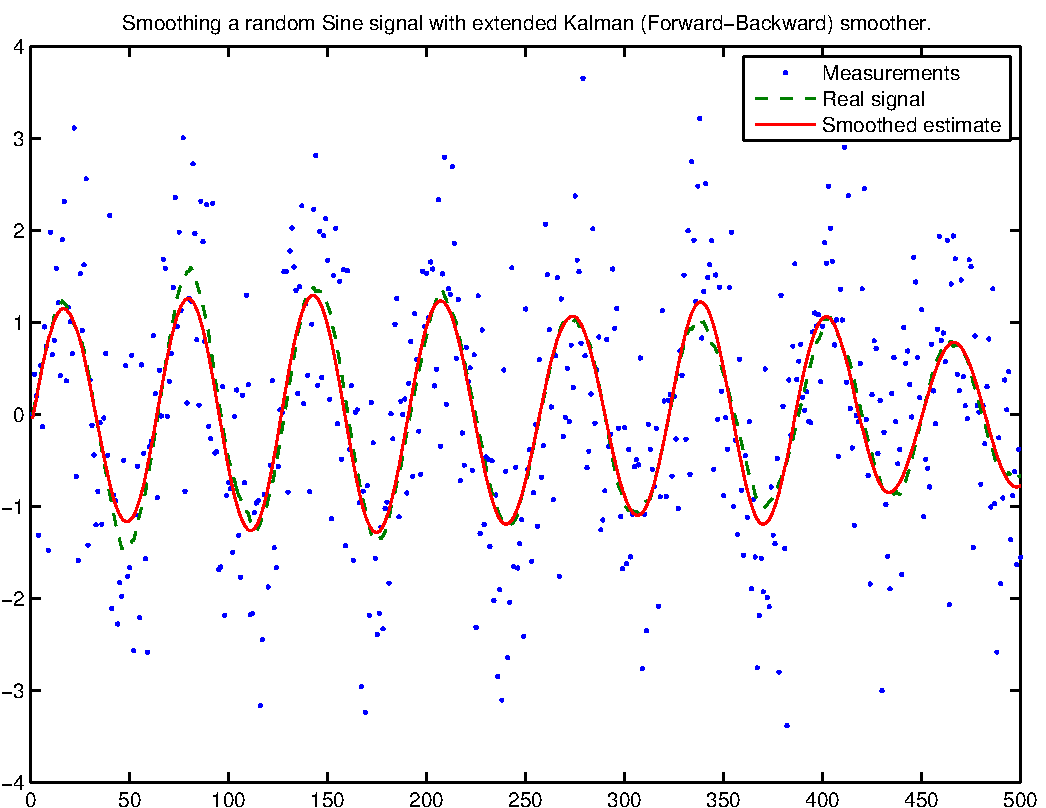
\includegraphics[width=11cm]{pics/demo2_f3}
\caption{Smoothed estimate of the sine signal using a combination of
two extended Kalman filters.}
\label{fig:example2_3}
\end{center}
\end{figure}


\begin{table}
\begin{center}
\begin{tabular}{|l|l|l|l|l|l|} \hline {\it Method}&{\it
RMSE[$\theta$]}&{\it RMSE[$\omega$]}&{\it RMSE[$a$]}& {\it
RMSE[$y$]}\\ \hline EKF1 & 0.64 & 0.53 & 0.40 & 0.24 \\ ERTS1& 0.52 &
0.31 & 0.33 & 0.15 \\ ETF1& 0.53 & 0.31 & 0.34 & 0.15 \\ EKF2 & 0.34 &
0.54 & 0.31 & 0.29 \\ ERTS2& 0.24 & 0.30 & 0.18 & 0.15 \\ ETF2& 0.24 &
0.30 & 0.18 & 0.15 \\ UKF & 0.59 & 0.56 & 0.39 & 0.27 \\ URTS & 0.45 &
0.30 & 0.30 & 0.15 \\ \hline
\end{tabular}
\caption{RMSEs of estimating the random sinusoid over 100 Monte Carlo
simulations.}
\label{table:sine_errors}
\end{center}
\end{table}



%%%%%%%%%%%%%%%%%%%%%%%%%%%%%%%%%%%%%%%%%%%%%%%%%%%%%%%%%%%%%%%%%%%%%%%%%%%%%%
%
\section{Unscented Kalman Filter}
%
%%%%%%%%%%%%%%%%%%%%%%%%%%%%%%%%%%%%%%%%%%%%%%%%%%%%%%%%%%%%%%%%%%%%%%%%%%%%%%

\subsection{Unscented Transform}

Like Taylor series based approximation presented above also the {\it
unscented transform} (UT) \citep{Julier+Uhlmann+Durrant-Whyte:1995, Julier+Uhlmann:2004, Wan+Merwe:2001} can be used for forming a Gaussian approximation to
the joint distribution of random variables $\vec{x}$ and $\vec{y}$,
which are defined with equations (\ref{eq:trans_g}). In UT we
deterministically choose a fixed number of sigma points, which capture
the desired moments (at least mean and covariance) of the original
distribution of $\vec{x}$ exactly. After that we propagate the sigma
points through the non-linear function $\vec{g}$ and estimate the
moments of the transformed variable from them.

The advantage of UT over the Taylor series based approximation is that
UT is better at capturing the higher order moments caused by the
non-linear transform, as discussed in \citep{Julier+Uhlmann:2004}. Also
the Jacobian and Hessian matrices are not needed, so the estimation
procedure is in general easier and less error-prone.
 
The unscented transform can be used to provide a Gaussian
approximation for the joint distribution of variables $\vec{x}$ and
$\vec{y}$ of the form
%
  \begin{equation}
     \begin{pmatrix} \vec{x} \\ \vec{y}
     \end{pmatrix} \sim \N\left(
     \begin{pmatrix} \vec{m} \\ \vecmu_U
     \end{pmatrix},
     \begin{pmatrix} \vec{P} & \vec{C}_U \\ \vec{C}_U^T & \mat{S}_U
     \end{pmatrix} \right).
  \end{equation}
%
The (nonaugmented) transformation is done as follows:
%
\begin{enumerate}
\item Compute the set of $2n+1$ sigma points from the columns of the
matrix $\sqrt{(n + \lambda) \, \mat{P}}$:
%
  \begin{equation}
  \begin{split} \vec{x}^{(0)} &= \vec{m} \\ \vec{x}^{(i)} &= \vec{m} +
\left[\sqrt{(n + \lambda) \, \mat{P}}\right]_i, \quad i=1,\ldots,n \\
\vec{x}^{(i)} &= \vec{m} - \left[\sqrt{(n + \lambda) \,
\mat{P}}\right]_i, \quad i=n+1,\ldots,2n
  \end{split}
  \label{eq:ut_sigmas}
  \end{equation}
%
  and the associated weights:
%
  \begin{equation}
  \begin{split} W^{(0)}_m &= \lambda / (n + \lambda) \\ W^{(0)}_c &=
\lambda / (n + \lambda) + (1 - \alpha^2 + \beta) \\ W^{(i)}_m &= 1 /
\{ 2(n + \lambda) \}, \quad i=1,\ldots,2n \\ W^{(i)}_c &= 1 / \{ 2(n +
\lambda) \}, \quad i=1,\ldots,2n.
  \end{split} \label{eq:ut_weights}
  \end{equation}
%
  Parameter $\lambda$ is a scaling parameter, which is defined as
%
  \begin{equation} \lambda = \alpha^2 \, (n + \kappa) - n.
  \end{equation}
 % 
  The positive constants $\alpha$, $\beta$ and $\kappa$ are used as
parameters of the method.

\item Propagate each of the sigma points through non-linearity as
%
  \begin{equation} \vec{y}^{(i)} = \vec{g}(\vec{x}^{(i)}), \quad
i=0,\ldots,2n.
  \label{eq:sigma_g}
  \end{equation}

\item Calculate the mean and covariance estimates for $\vec{y}$ as
%
  \begin{align} \vecmu_U &\approx \sum_{i=0}^{2n} W^{(i)}_m \,
\vec{y}^{(i)} \\ \mat{S}_U &\approx \sum_{i=0}^{2n} W^{(i)}_c \,
(\vec{y}^{(i)} - \vecmu_U) \, (\vec{y}^{(i)} - \vecmu_U)^T.
  \end{align}
  
\item Estimate the cross-covariance between $\vec{x}$ and $\vec{y}$ as
%
  \begin{equation} \mat{C}_U \approx \sum_{i=0}^{2n} W^{(i)}_c \,
(\vec{x}^{(i)} - \vec{m}) \, (\vec{y}^{(i)} - \vecmu_U)^T.
  \end{equation}
\end{enumerate}
%

The square root of positive definite matrix $\mat{P}$ is defined as
$\mat{A} = \sqrt{\mat{P}}$, where
%
\begin{equation}
%
\mat{P} = \mat{A} \mat{A}^T.
%
\end{equation}
%
To calculate the matrix $\mat{A}$ we can use, for example, lower
triangular matrix of the Cholesky factorialization, which can be
computed with built-in Matlab function \texttt{chol}. For convience,
we have provided a function (\texttt{schol}, which computes the factorialization also for
positive semidefinite matrices.


\subsection{The Matrix Form of UT}

The unscented transform described above can be written conviently in
matrix form as follows:
%
\begin{align} \mat{X} &=
      \begin{bmatrix} \vec{m} & \cdots & \vec{m} \end{bmatrix} +
\sqrt{c}
      \begin{bmatrix} \vec{0} & \sqrt{\mat{P}} & -\sqrt{\mat{P}}
      \end{bmatrix} \label{eq:ut_x1} \\ \mat{Y} &= \vec{g}(\mat{X})
\label{eq:ukf_x2} \\ \vecmu_U &= \mat{Y} \, \mat{w}_m \label{eq:ut_mu}
\\ \mat{S}_U &= \mat{Y} \, \mat{W} \, \mat{Y}^T \label{eq:ut_s} \\
\mat{C}_U &= \mat{X} \, \mat{W} \, \mat{Y}^T, \label{eq:ut_c}
\end{align}
%
where $\mat{X}$ is the matrix of sigma points, function
$\vec{g}(\cdot)$ is applied to each column of the argument matrix
separately, $c = \alpha^2 \, (n + \kappa)$, and vector $\vec{w}_m$ and
matrix $\mat{W}$ are defined as follows:
%
\begin{align} \vec{w}_m &= \begin{bmatrix} W^{(0)}_m & \cdots &
W^{(2n)}_m
   \end{bmatrix}^T \label{eq:vec_wm} \\ \mat{W} &= \left(\mat{I} -
     \begin{bmatrix} \vec{w}_m & \cdots & \vec{w}_m
     \end{bmatrix} \right) \, \nonumber \\ &\times \diag(W^{(0)}_c
\cdots W^{(2n)}_c) \, \nonumber \\ &\times \left(\mat{I} -
     \begin{bmatrix} \vec{w}_m & \cdots & \vec{w}_m
     \end{bmatrix} \right)^T.
   \label{eq:mat_w}
\end{align}
%
See (Särkkä, 2006) for proof for this.

%%%%%%%%%%%%%%%%%%%%%%%%%%%%%%%%%%%%%%%%%%%%%%%%%%%%%%%%%%%%%%%%%%%%%%%%%%%%%%
%
\subsection{Unscented Kalman Filter}
%
%%%%%%%%%%%%%%%%%%%%%%%%%%%%%%%%%%%%%%%%%%%%%%%%%%%%%%%%%%%%%%%%%%%%%%%%%%%%%%

The {\it unscented Kalman filter} (UKF) \citep{Julier+Uhlmann+Durrant-Whyte:1995, Julier+Uhlmann:2004, Wan+Merwe:2001} makes use of the {\it
unscented transform} described above to give a Gaussian approximation
to the filtering solutions of non-linear optimal filtering problems of
form (same as eq. (\ref{eq:nonlinear_prob}), but restated here for
convience)
%
\begin{equation}
\begin{split} \vec{x}_{k} &= \vec{f}(\vec{x}_{k-1},k-1) +
\vec{q}_{k-1} \\ \vec{y}_{k} &= \vec{h}(\vec{x}_{k},k) + \vec{r}_{k},
\end{split}
\end{equation}
%
where $\vec{x}_k \in \spc{R}^n$ is the state, $\vec{y}_k \in
\spc{R}^m$ is the measurement, $\vec{q}_{k-1} \sim
\N(\vec{0},\mat{Q}_{k-1})$ is the Gaussian process noise, and
$\vec{r}_{k} \sim \N(\vec{0},\mat{R}_{k})$ is the Gaussian measurement
noise.

Using the matrix form of UT described above the {\it prediction} and
{\it update} steps of the UKF can computed as follows:
%
\begin{itemize}
\item {\em Prediction:} Compute the predicted state mean $\vec{m}^-_k$
and the predicted covariance $\mat{P}^-_k$ as

%
\begin{equation}
\begin{split} \mat{X}_{k-1} &=
      \begin{bmatrix} \vec{m}_{k-1} & \cdots & \vec{m}_{k-1}
\end{bmatrix} + \sqrt{c}
      \begin{bmatrix} \vec{0} & \sqrt{\mat{P}_{k-1}} &
-\sqrt{\mat{P}_{k-1}}
      \end{bmatrix} \\ \hat{\mat{X}}_{k} &= \vec{f}(\mat{X}_{k-1},k-1)
\\ \vec{m}^-_{k} &= \hat{\mat{X}}_{k} \, \mat{w}_m \\ \mat{P}^-_{k} &=
\hat{\mat{X}}_{k} \, \mat{W} \, [ \hat{\mat{X}}_{k} ]^T +
\mat{Q}_{k-1}.
\end{split} \label{eq:ukf1_predict}
\end{equation}
%
\item {\em Update:} Compute the predicted mean $\vecmu_k$ and
covariance of the measurement $\mat{S}_k$, and the cross-covariance of
the state and measurement $\mat{C}_k$:
%
\begin{equation}
\begin{split} \mat{X}^-_k &=
      \begin{bmatrix} \vec{m}^-_k & \cdots & \vec{m}^-_k \end{bmatrix}
+ \sqrt{c}
      \begin{bmatrix} \vec{0} & \sqrt{\mat{P}^-_k} &
-\sqrt{\mat{P}^-_k}
      \end{bmatrix} \\ \mat{Y}^-_k &= \vec{h}(\mat{X}^-_k,k) \\
\vec{\mu}_k &= \mat{Y}^-_k \, \mat{w}_m \\ \mat{S}_k &= \mat{Y}^-_k \,
\mat{W} \, [\mat{Y}^-_k]^T + \mat{R}_{k} \\ \mat{C}_k &= \mat{X}^-_k
\, \mat{W} \, [\mat{Y}^-_k]^T.
\end{split}
\label{eq:ukf1_update1}
\end{equation}
%

Then compute the filter gain $\mat{K}_k$ and the updated state mean
$\vec{m}_k$ and covariance $\mat{P}_k$:
%
\begin{equation}
\begin{split} \mat{K}_k &= \mat{C}_k \, \mat{S}_k^{-1} \\ \vec{m}_k &=
\vec{m}^-_k + \mat{K}_k \, \left[ \vec{y}_k - \vecmu_k \right] \\
\mat{P}_k &= \mat{P}^-_k - \mat{K}_k \, \mat{S}_k \, \mat{K}_k^T.
\end{split}
\label{eq:ukf1_update2}
\end{equation}
\end{itemize}

The prediction and update steps of the nonaugmented UKF can be
computed with functions \texttt{ukf\_predict1} and
\texttt{ukf\_update1}, respectively.

\subsection{Augmented UKF}

It is possible to modify the UKF procedure described above by forming
an {\it augmented} state variable, which concatenates the state and
noise components together, so that the effect of process and
measurement noises can be used to better capture the odd-order moment
information. This requires that the sigma points generated during the
predict step are also used in the update step, so that the effect of
noise terms are truly propagated through the nonlinearity \citep{Wu+Hu+Wu+Hu:2005}. If, however, we generate new sigma points in the update step
the augmented approach give the same results as the nonaugmented, if
we had assumed that the noises were additive. If the noises are not
additive the augmented version should produce more accurate estimates
than the nonaugmented version, even if new sigma points are created
during the update step.

The {\it prediction} and {\it update} steps of the augmented UKF in
matrix form are as follows:
%
\begin{itemize}
\item {\em Prediction:} Form a matrix of sigma points of the augmented
state variable \\$\tilde{\vec{x}}_{k-1} =
\begin{bmatrix} \vec{x}_{k-1}^T & \vec{q}_{k-1}^T & \vec{r}_{k-1}^T
\end{bmatrix}^T$ as
%
\begin{equation}
%
\mat{\tilde{X}}_{k-1} =
   \begin{bmatrix} \tilde{\vec{m}}_{k-1} & \cdots &
\tilde{\vec{m}}_{k-1} \end{bmatrix} + \sqrt{c}
   \begin{bmatrix} \vec{0} & \sqrt{\tilde{\mat{P}}_{k-1}} &
-\sqrt{\tilde{\mat{P}}_{k-1}}
   \end{bmatrix},
%
\label{eq:ukf2_predict1}
\end{equation}
%
where
%
\begin{equation}
%
\tilde{\vec{m}}_{k-1} = \begin{bmatrix} \vec{m}_{k-1}^T & \vec{0} &
\vec{0} \end{bmatrix}^T
%
\text{ and }
%
\tilde{\mat{P}}_{k-1} =
\begin{bmatrix} \mat{P_{k-1}} & \mat{0} & \mat{0} \\ \mat{0} &
\mat{Q}_{k-1} & \mat{0} \\ \mat{0} & \mat{0} & \mat{R}_{k-1} \\
\end{bmatrix}.
%
\label{eq:ukf2_predict2}
\end{equation}

Then compute the predicted state mean $\vec{m}^-_k$ and the predicted
covariance $\mat{P}^-_k$ as
%
\begin{equation}
\begin{split} \hat{\mat{X}}_{k} &=
\vec{f}(\mat{X^x}_{k-1},\mat{X^q}_{k-1},k-1) \\ \vec{m}^-_{k} &=
\hat{\mat{X}}_{k} \, \mat{w}_m \\ \mat{P}^-_{k} &= \hat{\mat{X}}_{k}
\, \mat{W} \, [ \hat{\mat{X}}_{k} ]^T,
\end{split}
\label{eq:ukf2_predict3}
\end{equation}
%
where we have denoted the components of sigma points which correspond
to actual state variables and process noise with matrices
$\mat{X}^x_{k-1}$ and $\mat{X}^q_{k-1}$, respectively. The state
transition function $\vec{f}$ is also augmented to incorporate the
effect of process noise, which is now passed to the function as a
second parameter. In additive noise case the process noise is directly
added to the state variables, but other forms of noise effect are now
also allowed.

%
\item {\em Update:} Compute the predicted mean $\vecmu_k$ and
covariance of the measurement $\mat{S}_k$, and the cross-covariance of
the state and measurement $\mat{C}_k$:
%
\begin{equation}
\begin{split} \mat{Y}^-_k &=
\vec{h}(\hat{\mat{X}}_k,\mat{X}^r_{k-1},k) \\ \vec{\mu}_k &=
\mat{Y}^-_k \, \mat{w}_m \\ \mat{S}_k &= \mat{Y}^-_k \, \mat{W} \,
[\mat{Y}^-_k]^T \\ \mat{C}_k &= \hat{\mat{X}}_k \, \mat{W} \,
[\mat{Y}^-_k]^T,
\end{split}
\label{eq:ukf2_update1}
\end{equation}
%
where we have denoted the component of sigma points corresponding to
measurement noise with matrix $\mat{X}^r_{k-1}$. Like the state
transition function $\vec{f}$ also the measurement function $\vec{h}$
is now augmented to incorporate the effect of measurement noise, which
is passed as a second parameter to the function.

Then compute the filter gain $\mat{K}_k$ and the updated state mean
$\vec{m}_k$ and covariance $\mat{P}_k$:
%
\begin{equation}
\begin{split} \mat{K}_k &= \mat{C}_k \, \mat{S}_k^{-1} \\ \vec{m}_k &=
\vec{m}^-_k + \mat{K}_k \, \left[ \vec{y}_k - \vecmu_k \right] \\
\mat{P}_k &= \mat{P}^-_k - \mat{K}_k \, \mat{S}_k \, \mat{K}_k^T.
\end{split}
\label{eq:ukf2_update2}
\end{equation}
\end{itemize}
%

Note that nonaugmented form UKF is computationally less demanding than
augmented form UKF, because it creates a smaller number of sigma
points during the filtering procedure. Thus, the usage of the
nonaugmented version should be preferred over the nonaugmented
version, if the propagation of noise terms doesn't improve the
accuracy of the estimates.

The prediction and update steps of the augmented UKF can be computed
with functions \texttt{ukf\_predict3} and \texttt{ukf\_update3},
respectively. These functions concatenates the state variables,
process and measurements noises to the augmented variables, as was
done above.

It is also possible to separately concatenate only the state variables
and process noises during prediction step and state variables and
measurement noises during update step. Filtering solution based on
this formulation can be computed with functions \texttt{ukf\_predict2}
and \texttt{ukf\_update2}. However, these functions create new sigma
points during the update step in addition to ones created during
prediction step, and hence the higher moments might not get captured
so effectively in cases, where the noise terms are additive.


%%%%%%%%%%%%%%%%%%%%%%%%%%%%%%%%%%%%%%%%%%%%%%%%%%%%%%%%%%%%%%%%%%%%%%%%%%%%%%
%
\subsection{Unscented Kalman Smoother}
%
%%%%%%%%%%%%%%%%%%%%%%%%%%%%%%%%%%%%%%%%%%%%%%%%%%%%%%%%%%%%%%%%%%%%%%%%%%%%%%

The Rauch-Rung-Striebel type smoother using the unscented
transformation \citep{Sarkka:2008} can be used for computing a Gaussian
approximation to the smoothing distribution of the step $k$:
%
\begin{equation}
%
p(\vec{x}_k|\vec{y}_{1:T}) \sim N(\vec{x}_k|\vec{m}_k^s,\mat{P}_k^s),
%
\end{equation}
% 
as follows (using again the matrix form):
%
\begin{itemize}
%
\item Form a matrix of sigma points of the augmented state variable
$\tilde{\vec{x}}_{k-1} =
\begin{bmatrix} \vec{x}_{k-1}^T & \vec{q}_{k-1}^T \end{bmatrix}^T$ as
%
\begin{equation}
%
\mat{\tilde{X}}_{k-1} =
   \begin{bmatrix} \tilde{\vec{m}}_{k-1} & \cdots &
\tilde{\vec{m}}_{k-1} \end{bmatrix} + \sqrt{c}
   \begin{bmatrix} \vec{0} & \sqrt{\tilde{\mat{P}}_{k-1}} &
-\sqrt{\tilde{\mat{P}}_{k-1}}
   \end{bmatrix},
%
\label{eq:urts1}
\end{equation}
%
where
%
\begin{equation}
%
\tilde{\vec{m}}_{k-1} = \begin{bmatrix} \vec{m}_{k-1}^T & \vec{0}
\end{bmatrix}^T
%
\text{ and }
%
\tilde{\mat{P}}_{k-1} =
\begin{bmatrix} \mat{P_{k-1}} & \mat{0} \\ \mat{0} & \mat{Q}_{k-1} \\
\end{bmatrix}.
\label{eq:urts2}
\end{equation}
%
\item Propagate the sigma points through the dynamic model:
%
\begin{equation}
%
\tilde{\mat{X}}_{k+1}^- =
\vec{f}(\tilde{\mat{X}}^x_{k},\tilde{\mat{X}}^q_{k},k),
%
\label{eq:urts3}
\end{equation}
% 
where $\tilde{\mat{X}}^x_{k}$ and $\tilde{\mat{X}}^q_{k}$ denotes the
parts of sigma points, which correspond to $\vec{x}_k$ and
$\vec{q}_k$, respectively.

\item Compute the predicted mean $\vec{m}^-_{k+1}$, covariance
$\mat{P}^-_{k+1}$ and cross-covariance $\mat{C}_{k+1}$:
\begin{equation}
\begin{split} \vec{m}^-_{k+1} &= \tilde{\mat{X}}_{k+1}^{-x} \,
\mat{w}_m \\ \mat{P}^-_{k+1} &= \tilde{\mat{X}}_{k+1}^{-x} \, \mat{W}
\, [\tilde{\mat{X}}_{k+1}^{-x}]^T \\ \mat{C}_{k+1} &=
\tilde{\mat{X}}_{k+1}^{-x} \, \mat{W} \, [\tilde{\mat{X}}^x_{k}]^T,
\end{split}
\label{eq:urts4}
\end{equation}
%
where $\tilde{\mat{X}}_{k+1}^{-x}$ denotes the part of propagated
sigma points $\tilde{\mat{X}}_{k+1}^-$, which corresponds to
$\vec{x}_k$.
%
\item Compute the smoother gain $\mat{D}_k$, the smoothed mean
$\vec{m}_k^s$ and the covariance $\mat{P}_k^s$:
\begin{equation}
\begin{split} \mat{D}_k & = \mat{C}_{k+1} [\mat{P}_{k+1}^-]^{-1} \\
\vec{m}_k^s & = \vec{m}_k + \mat{D}_k [\vec{m}^s_{k+1} -
\vec{m}_{k+1}^-] \\ \mat{P}_k^s & = \mat{P}_k + \mat{D}_k
[\mat{P}^s_{k+1} - \mat{P}_{k+1}^-] \mat{D}_k^T.
\end{split}
\label{eq:urts5}
\end{equation}

\end{itemize}
%

The smoothing solution of this augmented type RTS smoother can be
computed with function \texttt{urts\_smooth2}. Also a nonaugmented
version of this type smoother has been implemented, and a smoothing
solution with that can be computed with function
\texttt{urts\_smooth1}.



\newpage \clearpage

%%%%%%%%%%%%%%%%%%%%%%%%%%%%%%%%%%%%%%%%%%%%%%%%%%%%%%%%%%%%%%%%%%%%%%%%%%%%%%
%
   % Cubature Methods in non-linear Kalman filtering and smoothing
%
   % These sections were added to the toolbox documentation originally in summer 2010.
%    
   % Arno Solin, 2010
%
%%%%%%%%%%%%%%%%%%%%%%%%%%%%%%%%%%%%%%%%%%%%%%%%%%%%%%%%%%%%%%%%%%%%%%%%%%%%%%




%%%%%%%%%%%%%%%%%%%%%%%%%%%%%%%%%%%%%%%%%%%%%%%%%%%%%%%%%%%%%%%%%%%%%%%%%%%%%%
%
\section{Gauss-Hermite Kalman Filter}
%
%%%%%%%%%%%%%%%%%%%%%%%%%%%%%%%%%%%%%%%%%%%%%%%%%%%%%%%%%%%%%%%%%%%%%%%%%%%%%%

\subsection{Gauss-Hermite Cubature Transformation}

To unify many of the filter variants, handling the non-linearities may be brought together to a common formulation. In Gaussian optimal filtering --- also called assumed density filtering --- the filtering equations follow the assumption that the filtering distributions are indeed Gaussian \citep{Maybeck:1982, Ito+Xiong:2000}. %\citep{maybeck1982,ito2000}.

Using this setting the linear Kalman filter equations can now be adapted to the non-linear state-space model. Desired moments (at least mean and covariance) of the original distribution of $\vec{x}$ can be captured exactly by calculating the integrals

\begin{align}%
\begin{split} \label{eqCh2integral1}
    \bmu_U &= \int \vec{f}(\vec{x})\,\N(\vec{x} \mid \vec{m},\,\vec{P}) \diff \vec{x} \\
    \vec{S}_U &= \int \left(\vec{f}(\vec{x}) - \bmu_U\right) \left(\vec{f}(\vec{x}) - \bmu_U\right)\T 
     \times \N(\vec{x} \mid \vec{m},\,\vec{P}) \diff \vec{x}.
\end{split}%
\end{align}

These integrals can be evaluated with practically any analytical or numerical integration method. The Gauss--Hermite quadrature rule is a one-dimensional weighted sum approximation method for solving special integrals of the previous form in a Gaussian kernel with an infinite domain. More specifically the Gauss--Hermite quadrature can be applied to integrals of form

\begin{equation} \label{eqGaussHermite1D}
    \int_{-\infty}^\infty f(x)\,\exp(-x^2) \diff x \approx \sum_{i=1}^m w_i\,f(x_i),
\end{equation}

\noindent%
where $x_i$ are the sample points and $w_i$ the associated weights to use for the approximation. The sample points $x_i, i=1,\ldots,m,$ are roots of special orthogonal polynomials, namely the Hermite polynomials. The Hermite polynomial of degree $p$ is denoted with $H_p(x)$ \citep[see][for details]{Abramowitz+Stegun:1964}. The weights $w_i$ are given by

\begin{equation} \label{eqGaussHermiteWeights}
    w_i = \frac{2^{p-1}p!\sqrt{\pi}}{p^2[H_{p-1}(x_i)]^2}.
\end{equation}

The univariate integral approximation needs to be extended to be able to suit the multivariate case. As \citet{Wu+Hu+Wu+Hu:2006}  argue, the most natural approach to grasp a multiple integral is to treat it as a sequence of nested univariate integrals and then use a univariate quadrature rule repeatedly. To extend this one-dimensional integration method to multi-dimensional integrals of form

\begin{equation} \label{eqGaussHermiteND}
    \int_{\mathbb{R}^n} f(\vec{x})\,\exp(-\vec{x}\T\vec{x}) \diff \vec{x} \approx \sum_{i=1}^m w_i\,f(\vec{x}_i),
\end{equation}

\noindent%
we first simply form the one-dimensional quadrature rule with respect to the first dimension, then with respect to the second dimension and so on \citep{Cools:1997}. We get the multidimensional Gauss--Hermite cubature rule by writing

\begin{align*}
    & \sum_{i_1} w_{i_1} \int f(x_1^{i_1},x_2, \ldots, x_n) \exp(-x_2^2 -x_3^2 \ldots -x_n^2) \diff x_2 \ldots \diff x_n \\
    =& \sum_{i_1,i_2} w_{i_1} w_{i_2} \int f(x_1^{i_1},x_2^{i_2}, \ldots, x_n) \exp(-x_3^2 \ldots -x_n^2) \diff x_3 \ldots \diff x_n \\
    =& \sum_{i_1,i_2,\ldots,i_n} w_{i_1} w_{i_2} \cdots  w_{i_n} \, f(x_1^{i_1},x_2^{i_2}, \ldots, x_n^{i_n}),
\end{align*}

\noindent%
which is basically what we wanted in Equation~\eqref{eqGaussHermiteND}. This gives us the \emph{product rule} that simply extends the one-dimensional quadrature point set of $p$ points in one dimension to a lattice of $p^n$ cubature points in $n$ dimensions. The weights for these Gauss--Hermite cubature points are calculated by the product of the corresponding one-dimensional weights.

Finally, by making a change of variable $\vec{x} = \sqrt{2}\sqrt{\vec{\Sigma}} + \bmu$ we get the Gauss--Hermite weighted sum approximation for a multivariate Gaussian integral, where $\bmu$ is the mean and $\bSigma$ is the covariance of the Gaussian. The square root of the covariance matrix, denoted $\sqrt{\bSigma}$, is  a matrix such that $\bSigma = \sqrt{\bSigma}\sqrt{\bSigma}\T$.

\begin{equation}
    \int_{\mathbb{R}^n} \vec{f}(\vec{x})\,\N(\vec{x} \mid \bmu,\, \vec{\Sigma})\diff\vec{x} 
    \approx \sum_{i_1, i_2, \ldots, i_n} w_{i_1, i_2, \ldots, i_n} \, f\left(\sqrt{\vec{\Sigma}}\, \boldsymbol{\xi}_{i_1, i_2, \ldots, i_n} +\bmu \right),
\end{equation}

\noindent%
where the weight $w_{i_1, i_2, \ldots, i_n} = {1 \over \pi^{n/2}} w_{i_1} \cdot w_{i_2} \cdots w_{i_n}$ is given by using the one-dimensional weights, and the points are given by the Cartesian product $\boldsymbol{\xi}_{i_1, i_2, \ldots, i_n} = \sqrt{2} \, (x_{i_1}, x_{i_2}, \ldots, x_{i_n})$, where $x_i$ is the $i$th one-dimensional quadrature point. 

%% The curse of dimensionality
The extension of the Gauss--Hermite quadrature rule to an $n$-dimensional cubature rule by using the product rule lattice approach yields a rather good numerical integration method that is exact for monomials $\prod_{i=1}^n x_i^{k_i} $ with $k_i \leq 2p - 1$ \citep{Wu+Hu+Wu+Hu:2006}. However, the number of cubature points grows exponentially as the number of dimensions increases. Due to this flaw the rule is not practical in applications with many dimensions. This problem is called the \emph{curse of dimensionality}.












%%%%%%%%%%%%%%%%%%%%%%%%%%%%%%%%%%%%%%%%%%%%%%%%%%%%%%%%%%%%%%%%%%%%%%%%%%%%%%
%
\subsection{Gauss-Hermite Kalman Filter}
%
%%%%%%%%%%%%%%%%%%%%%%%%%%%%%%%%%%%%%%%%%%%%%%%%%%%%%%%%%%%%%%%%%%%%%%%%%%%%%%

The Gauss--Hermite Kalman filter (GHKF) algorithm of degree $p$ is presented below. At time $k = 1,\ldots,T$ assume the posterior density function $ p(\vec{x}_{k-1} \mid \vec{y}_{k-1}) = \N(\vec{m}_{k-1 \mid k-1},\vec{P}_{k-1 \mid k-1})$ is known.


%% The Prediction step
\textbf{Prediction step:}

\begin{enumerate}

  \item Find the roots $x_i, i=1,\ldots,p$, of the Hermite polynomial $H_p(x)$.%

  \item Calculate the corresponding weights%
%
   $$ w_i = \frac{2^{p-1}p!}{p^2[H_{p-1}(x_i)]^2}. $$

  \item Use the product rule to expand the points to a $n$-dimensional lattice of $p^n$ points $\boldsymbol{\xi}_i, i=1,\ldots,p^n,$ with corresponding weights. 

  \item Propagate the cubature points. The matrix square root is the lower triangular cholesky factor.%
%
    $$ \vec{X}_{i,k-1 \mid k-1} = \sqrt{2 \vec{P}_{k-1 \mid k-1}} \boldsymbol{\xi}_i + \vec{m}_{k-1 \mid k-1}$$

  \item Evaluate the cubature points with the dynamic model function%
%
    $$ \vec{X}_{i,k \mid k-1}^* = \vec{f}(\vec{X}_{i,k-1 \mid k-1}). $$

  \item Estimate the predicted state mean%
%
    $$ \vec{m}_{k \mid k-1}  = \sum_{i=1}^{p^n} w_i \vec{X}_{i,k \mid k-1}^*. $$

  \item Estimate the predicted error covariance%
%
    $$ \vec{P}_{k \mid k-1} = \sum_{i=1}^{p^n} w_i \vec{X}_{i,k \mid k-1}^* \vec{X}_{i,k \mid k-1}^{*\mathsf{T}} - \vec{m}_{k \mid k-1} \vec{m}_{k \mid k-1}\T + \vec{Q}_{k-1}.$$ 

\end{enumerate}


%% The Update step
\noindent
\textbf{Update step:}

\begin{enumerate}

  \item Repeat steps 1--3 from earlier to get the $p^n$ cubature points and their weights. 

  \item Propagate the cubature points.%
%
    $$ \vec{X}_{i,k \mid k-1} = \sqrt{2 \vec{P}_{k \mid k-1}} \boldsymbol{\xi}_i + \vec{m}_{k \mid k-1}$$

  \item Evaluate the cubature points with the help of the measurement model function%
%
    $$ \vec{Y}_{i,k \mid k-1} = \vec{h}(\vec{X}_{i,k \mid k-1}). $$

  \item Estimate the predicted measurement%
%
    $$ \vec{\hat{y}}_{k \mid k-1} = \sum_{i=1}^{p^n} w_i \vec{Y}_{i,k \mid k-1}. $$

  \item Estimate the innovation covariance matrix%
%
    $$ \vec{S}_{k \mid k-1} = \sum_{i=1}^{p^n} w_i \vec{Y}_{i,k \mid k-1} \vec{Y}_{i,k \mid k-1}\T - \vec{\hat{y}}_{k \mid k-1} \vec{\hat{y}}_{k \mid k-1}\T + \vec{R}_k. $$
    
  \item Estimate the cross-covariance matrix%
%
    $$ \vec{P}_{xy,k \mid k-1} = \sum_{i=1}^{p^n} w_i \vec{X}_{i,k-1 \mid k-1} \vec{Y}_{i,k \mid k-1}\T - \vec{m}_{k \mid k-1} \vec{\hat{y}}_{k \mid k-1}\T.$$ 

  \item Calculate the Kalman gain term and the smoothed state mean and covariance%
%
  \begin{align*}
     \vec{K}_k = \vec{P}_{xy,k \mid k-1} \vec{S}_{k \mid k-1}^{-1} \\
     \vec{m}_{k \mid k} = \vec{m}_{k \mid k-1} + \vec{K}_k(\vec{y}_k - \vec{\hat{y}}_{k \mid k-1}) \\
     \vec{P}_{k \mid k} = \vec{P}_{k \mid k-1} - \vec{K}_k \vec{P}_{yy,k \mid k-1} \vec{K}_k\T. 
  \end{align*}
\end{enumerate}












%%%%%%%%%%%%%%%%%%%%%%%%%%%%%%%%%%%%%%%%%%%%%%%%%%%%%%%%%%%%%%%%%%%%%%%%%%%%%%
%
\subsection{Gauss-Hermite Kalman Smoother}
%
%%%%%%%%%%%%%%%%%%%%%%%%%%%%%%%%%%%%%%%%%%%%%%%%%%%%%%%%%%%%%%%%%%%%%%%%%%%%%%

The Gauss--Hermite Rauch--Tung--Striebel smoother (GHRTS) algorithm \citep{Sarkka+Hartikainen:2010} of degree $p$ is presented below. Assume the filtering result mean $\vec{m}_{k \mid k}$ and covariance $\vec{P}_{k \mid k}$ are known together with the smoothing result $ p(\vec{x}_{k+1} \mid \vec{y}_{1:T}) = \N(\vec{m}_{k+1 \mid T},\vec{P}_{k+1 \mid T})$.


%% Smoothing
\begin{enumerate}

  \item Find the roots $x_i, i=1,\ldots,p$, of the Hermite polynomial $H_p(x)$.%

  \item Calculate the corresponding weights%
%
   $$ w_i = \frac{2^{p-1}p!}{p^2[H_{p-1}(x_i)]^2}. $$

  \item Use the product rule to expand the points to a $n$-dimensional lattice of $p^n$ points $\boldsymbol{\xi}_i, i=1,\ldots,p^n,$ with corresponding weights.  

  \item Propagate the cubature points%
%
    $$ \vec{X}_{i,k \mid k} = \sqrt{2 \vec{P}_{k \mid k}} \boldsymbol{\xi}_i + \vec{m}_{k \mid k}. $$

  \item Evaluate the cubature points with the dynamic model function%
%
    $$ \vec{X}_{i,k+1 \mid k}^* = \vec{f}(\vec{X}_{i,k \mid k}). $$

  \item Estimate the predicted state mean%
%
    $$ \vec{m}_{k+1 \mid k}  = \sum_{i=1}^{p^n} w_i \vec{X}_{i,k+1 \mid k}^*. $$

  \item Estimate the predicted error covariance%
%
    $$ \vec{P}_{k+1 \mid k} = \sum_{i=1}^{p^n} w_i \vec{X}_{i,k+1 \mid k}^* \vec{X}_{i,k+1 \mid k}^{*\mathsf{T}} - \vec{m}_{k+1 \mid k} \vec{m}_{k+1 \mid k}\T + \vec{Q}_{k}.$$

  \item Estimate the cross-covariance matrix%
%
    $$ \vec{D}_{k , k+1} = {1 \over 2 n} \sum_{i=1}^{2 n} \big(\vec{X}_{i,k \mid k} - \vec{m}_{k \mid k}\big) \\ \big(\vec{X}_{i,k+1 \mid k}^* - \vec{m}_{k+1 \mid k}\big)\T. $$ 

  \item Calculate the gain term and the smoothed state mean and covariance%
%
  \begin{align*}
     \vec{C}_k &= \vec{D}_{k , k+1} \vec{P}_{k+1 \mid k}^{-1} \\
     \vec{m}_{k \mid T} &= \vec{m}_{k \mid k} + \vec{C}_k(\vec{m}_{k+1 \mid T} - \vec{m}_{k+1 \mid k}) \\
     \vec{P}_{k \mid T} &= \vec{P}_{k \mid k} + \vec{C}_k (\vec{P}_{k+1 \mid T} - \vec{P}_{k+1 \mid k}) \vec{C}_k\T.
  \end{align*}

\end{enumerate}














\newpage
%%%%%%%%%%%%%%%%%%%%%%%%%%%%%%%%%%%%%%%%%%%%%%%%%%%%%%%%%%%%%%%%%%%%%%%%%%%%%%
%
\section{Cubature Kalman Filter}
%
%%%%%%%%%%%%%%%%%%%%%%%%%%%%%%%%%%%%%%%%%%%%%%%%%%%%%%%%%%%%%%%%%%%%%%%%%%%%%%

\subsection{Spherical-Radial Cubature Transformation}

As in the Gauss--Hermite cubature rule based Gauss--Hermite transformation the spherical--radial cubature transformation utilizes the assumed density approach. The integrals that need to be solved are the same Gaussian integrals, but the numerical integration method differs from the product rule based Gauss--Hermite method.

The curse of dimensionality causes all product rules to be highly ineffective in integration regions with multiple dimensions. To mitigate this issue, we may seek alternative approaches to solving Gaussian integrals. The non-product rules differ from product based solutions by choosing the evaluation points directly from the domain of integration. That is, the points are not simply duplicated from one dimension to multiple dimensions, but directly chosen from the whole domain.

We constrain our interest to integrals of form

\begin{equation} \label{eqAlmostgaussian}
    \operatorname{I}(\vec{f}) = \int_{\mathbb{R}^n} f(\vec{x})\exp(-\vec{x}\T\vec{x})\diff\vec{x}.
\end{equation}

\noindent%
We make a change of variable from $\vec{x} \in \mathbb{R}^n$ to spherical coordinates, which lets us split the integrand into two: a radial integral

\begin{equation} \label{eqRadial}
    \operatorname{I}(\vec{f}) = \int_0^\infty \operatorname{S}(r) \, r^{n-1} \exp(-r^2) \diff r,
\end{equation}

\noindent%
and a spherical integral

\begin{equation} \label{eqSpherical}
    \operatorname{S}(r) = \int_{S_n} f(r\vec{y}) \diff\sigma(\vec{y}).
\end{equation}

The spherical integral~\eqref{eqSpherical} can be seen as a spherical integral with the unit weighting function $w(\vec{y}) \equiv 1$. Now the spherical and radial integral may be interpreted separately and computed with the spherical cubature rule and the Gaussian quadrature rule respectively.




In a fully symmetric cubature point set equally weighted points are symmetrically distributed around origin. A point $\vec{u}$ is called the \emph{generator} of such a set, if for the components of $\vec{u} = \begin{pmatrix} u_1,u_2,\ldots,u_r,0,\ldots,0 \end{pmatrix} \in \mathbb{R}^n$, $u_i \geq u_{i+1} > 0,\, i= 1,2,\ldots,(r-1)$. For example, we may denote $[\vec{1}] \in \mathbb{R}^2$ to represent the cubature point set 

\begin{equation*}
\left\{ 
  \begin{pmatrix}  1 \\  0  \end{pmatrix},
  \begin{pmatrix}  0 \\  1  \end{pmatrix},
  \begin{pmatrix} -1 \\  0  \end{pmatrix},
  \begin{pmatrix}  0 \\ -1  \end{pmatrix}
 \right\},
\end{equation*}

\noindent%
where the generator is $\begin{pmatrix} 1 & 0 \end{pmatrix}\T$.

To find the unknowns of a cubature rule of degree $d$, a set of moment equations have to be solved. This, however, may not be a simple task with increasing dimensions and polynomial degree. To reduce the size of the system of equations or the number of needed cubature points \citep{Arasaratnam+Haykin:2009} use the \emph{invariant theory} proposed by Sobolev \citep[see][]{Cools:1997}. The invariant theory discusses how to simplify the structure of a cubature rule by using the symmetries of the region of integration. The unit hypercube, the unit  hypersphere and the unit simplex all contain some symmetry.

Due to invariance theory \citep{Cools:1997} the integral~\eqref{eqSpherical} can be approximated by a third-degree spherical cubature rule that gives us the sum

\begin{equation} \label{eqSphericalSum}
    \int_{S_n} f(r\vec{y}) \diff\sigma(\vec{y}) \approx w \sum_{i=1}^{2n}\vec{f}([\vec{u}]_i).
\end{equation}

\noindent%
The point set $[\vec{u}]$ is invariant under permutations and sign changes, which means that a number of $2n$ cubature points are sufficient to approximate the integral. For the above choice, the monomials $y_1^{d_1}y_2^{d_2}\cdots y_n^{d_n}$, with the sum $\sum_{i=1}^n d_i$ being an odd integer, are integrated exactly.

To make this rule exact for all monomials up to degree three, we have to require the rule to be exact for the even dimensions $\sum_{i=1}^n d_i = \{0,2\}$. This can be accomplished by solving the unknown parameters for a monomial function of order $n=0$ and equivalently for a monomial function of order $n=2$. We consider the two functions $\vec{f}(\cdot)$ to be of form $\vec{f}(\vec{y})=1$, and $\vec{f}(\vec{y})=y_1^2$. This yields the pair of equations \citep{Arasaratnam:2009}.

\begin{align*}
    \vec{f}(\vec{y})&=1 :& 2nw &= \int_{S_n} \diff\sigma(\vec{y}) = A_n \\
    \vec{f}(\vec{y})&=y_1^2 :& 2wu^2 &= \int_{S_n} y_1^2 \diff\sigma(\vec{y}) = \frac{1}{n} A_n,
\end{align*}

\noindent%
where $A_n$ is the surface area of the $n$-dimensional unit sphere. Solving these equations yields $u^2 = 1$ and $w = \frac{A_n}{2n}$. Therefore the cubature points can be chosen so that they are located at the intersection of the unit sphere and its axes.







The radial integral defined in Equation~\eqref{eqRadial} can be transformed to a familiar Gauss--Laguerre form (see Abramowitz and Stegun, 1964) by making another change of variable, $t=r^2$, which yields

\begin{equation} \label{eqRadialChange}
    \int_0^\infty \operatorname{S}(r) \, r^{n-1} \exp(-r^2) \diff r = 
    {1 \over 2} \int_0^\infty \operatorname{\tilde{S}}(t) \, t^{{n \over 2}-1} \exp(-t) \diff t = \sum_{i=1}^m w_i \operatorname{\tilde{S}}(t_i),
\end{equation}

where $t_i$ is the $i$th root of \emph{Laguerre polynomial} $L_m(t)$ and the weights $w_i$ are given by \citep{Abramowitz+Stegun:1964} 

  $$w_i = {t_i \over (m+1)^2(L_{m+1}(t_i))^2}.$$

\noindent%
A first-degree Gauss--Laguerre rule is exact for $\operatorname{\tilde{S}}(t)=\{1,t\}$ (or equivalently $\operatorname{S}(r)=\{1,r^2\}$). Due to the properties of the spherical cubature rule presented earlier, the combined spherical--radial rule vanishes by symmetry for all odd degree polynomials. Hence, to have the spherical--radial rule to be exact for all polynomials up to degree three in $\vec{x} \in \mathbb{R}^n$ it is sufficient to use the first degree Gauss--Laguerre rule of the form \citep{Arasaratnam:2009}

\begin{equation*}
    \int_0^\infty \operatorname{\tilde{S}_i}(t) \, t^{{n \over 2}-1} \exp(-t) \diff t = 
    w_1 \operatorname{\tilde{S}_i}(t_1),\quad i=\{0,1\},
\end{equation*}

\noindent%
where $\operatorname{\tilde{S}_0}(t)=1$ and $\operatorname{\tilde{S}_1}(t)=t$. The corresponding moment equations show that the first-degree Gauss--Laguerre approximation is constructed using the point $t_1 = {n \over 2}$ and the weight $w_1 = \Gamma({n \over 2})$, where $\Gamma(\cdot)$ is the Gamma function. The final radial form approximation can be written using Equation~\eqref{eqRadialChange} in the form

\begin{equation} \label{eqRadialFinal}
    \int_0^\infty \operatorname{S}(r) \, r^{n-1} \exp(-r^2) \diff r \approx
    {1 \over 2}\, \Gamma\left({n \over 2}\right)\operatorname{S}\left( \sqrt{{n \over 2}} \right).
\end{equation}

Now we have an approximation for the spherical integral in Equation~\eqref{eqSphericalSum}, where the third-degree rule is acquired by the cubature point set $[\vec{1}]$ and weight ${A_n \over 2n}$. Here the surface area $A_n$ of the $n-1$ hypersphere equals $2 {\pi^{n/2} \over \Gamma(n/2)}$, where $\Gamma(\cdot)$ is the Gamma function. 
By applying the results derived for the spherical and radial integral, we may combine Equations~\eqref{eqSphericalSum} and~\eqref{eqRadialFinal} to construct a third-degree cubature approximation for \eqref{eqAlmostgaussian}, which yields the elegant solution

\begin{equation*}
    \operatorname{I}(\vec{f}) 
    \approx {\sqrt{\pi^n} \over 2n} \sum_{i=1}^{2n} \vec{f}\left( \sqrt{{n \over 2}} [\vec{1}]_i \right).
\end{equation*}

By making a change of variable we get the third-degree spherical--radial cubature rule for an arbitrary integral that is of form \emph{non-linear function $\times$ Gaussian}. It can be written as

\begin{equation*}
    \int_{\mathbb{R}^n} \vec{f}(\vec{x})\,\N(\vec{x} \mid \bmu,\, \vec{\Sigma})\diff\vec{x} 
    \approx \sum_{i=1}^{2n} w_i \vec{f}\left(\sqrt{\vec{\Sigma}}\, \boldsymbol{\xi}_i +\bmu \right),
\end{equation*}

where the cubature points are $\boldsymbol{\xi}_i = \sqrt{n} [\vec{1}]_i$, the corresponding (equal) weights $w_i = {1 \over 2n}$ and the points $[\vec{1}]_i$ from the intersections between the Cartesian axes and the $n$-dimensional unit hypersphere.

Note that the spherical--radial cubature transform coincide with the result of the unscented transform when the unscented transform is done with parameter values $\alpha = \pm 1$, $\beta = 0$ and $\kappa = 0$.



%%%%%%%%%%%%%%%%%%%%%%%%%%%%%%%%%%%%%%%%%%%%%%%%%%%%%%%%%%%%%%%%%%%%%%%%%%%%%%
%
\subsection{Spherical-Radial Cubature Kalman Filter}
%
%%%%%%%%%%%%%%%%%%%%%%%%%%%%%%%%%%%%%%%%%%%%%%%%%%%%%%%%%%%%%%%%%%%%%%%%%%%%%%

The cubature Kalman filter (CKF) algorithm is presented below. At time $k = 1,\ldots,T$ assume the posterior density function $ p(\vec{x}_{k-1} \mid \vec{y}_{k-1}) = \N(\vec{m}_{k-1 \mid k-1},\vec{P}_{k-1 \mid k-1})$ is known.


%% The Prediction step
\textbf{Prediction step:}

\begin{enumerate}

  \item Draw cubature points $\boldsymbol{\xi}_i, i=1,\ldots,2n$ from the intersections of the $n$-dimensional unit sphere and the Cartesian axes. Scale them by $\sqrt{n}$. That is
%
    $$ \boldsymbol{\xi}_i =
	\begin{cases} 
	    \sqrt{n} \, e_i      & ,\: i = 1,\ldots,n \\
	    -\sqrt{n} \, e_{i-n} & ,\: i = n+1,\ldots,2n
	\end{cases}
 $$

  \item Propagate the cubature points. The matrix square root is the lower triangular cholesky factor.%
%
    $$ \vec{X}_{i,k-1 \mid k-1} = \sqrt{\vec{P}_{k-1 \mid k-1}} \boldsymbol{\xi}_i + \vec{m}_{k-1 \mid k-1}$$

  \item Evaluate the cubature points with the dynamic model function%
%
    $$ \vec{X}_{i,k \mid k-1}^* = \vec{f}(\vec{X}_{i,k-1 \mid k-1}). $$

  \item Estimate the predicted state mean%
%
    $$ \vec{m}_{k \mid k-1}  = {1 \over 2 n} \sum_{i=1}^{2 n} \vec{X}_{i,k \mid k-1}^*. $$

  \item Estimate the predicted error covariance%
%
    $$ \vec{P}_{k \mid k-1} = {1 \over 2 n} \sum_{i=1}^{2 n} \vec{X}_{i,k \mid k-1}^* \vec{X}_{i,k \mid k-1}^{*\mathsf{T}} - \vec{m}_{k \mid k-1} \vec{m}_{k \mid k-1}\T + \vec{Q}_{k-1}.$$ 

\end{enumerate}


%% The Update step
\noindent
\textbf{Update step:}

\begin{enumerate}

  \item Draw cubature points $\boldsymbol{\xi}_i, i=1,\ldots,2n$ from the intersections of the $n$-dimensional unit sphere and the Cartesian axes. Scale them by $\sqrt{n}$.

  \item Propagate the cubature points.%
%
    $$ \vec{X}_{i,k \mid k-1} = \sqrt{\vec{P}_{k \mid k-1}} \boldsymbol{\xi}_i + \vec{m}_{k \mid k-1}$$

  \item Evaluate the cubature points with the help of the measurement model function%
%
    $$ \vec{Y}_{i,k \mid k-1} = \vec{h}(\vec{X}_{i,k \mid k-1}). $$

  \item Estimate the predicted measurement%
%
    $$ \vec{\hat{y}}_{k \mid k-1} = {1 \over 2 n} \sum_{i=1}^{2 n} \vec{Y}_{i,k \mid k-1}. $$

  \item Estimate the innovation covariance matrix%
%
    $$ \vec{S}_{k \mid k-1} = {1 \over 2 n} \sum_{i=1}^{2 n} \vec{Y}_{i,k \mid k-1} \vec{Y}_{i,k \mid k-1}\T - \vec{\hat{y}}_{k \mid k-1} \vec{\hat{y}}_{k \mid k-1}\T + \vec{R}_k.$$

  \item Estimate the cross-covariance matrix%
%
    $$ \vec{P}_{xy,k \mid k-1} = {1 \over 2 n} \sum_{i=1}^{2 n} \vec{X}_{i,k-1 \mid k-1} \vec{Y}_{i,k \mid k-1}\T - \vec{m}_{k \mid k-1} \vec{\hat{y}}_{k \mid k-1}\T.$$ 

  \item Calculate the Kalman gain term and the smoothed state mean and covariance %
%
  \begin{align*}
     \vec{K}_k &= \vec{P}_{xy,k \mid k-1} \vec{S}_{k \mid k-1}^{-1} \\
     \vec{m}_{k \mid k} &= \vec{m}_{k \mid k-1} + \vec{K}_k(\vec{y}_k - \vec{\hat{y}}_{k} \\ 
     \vec{P}_{k \mid k} &= \vec{P}_{k \mid k-1} - \vec{K}_k \vec{P}_{yy,k \mid k-1} \vec{K}_k\T.
  \end{align*}
\end{enumerate}






%%%%%%%%%%%%%%%%%%%%%%%%%%%%%%%%%%%%%%%%%%%%%%%%%%%%%%%%%%%%%%%%%%%%%%%%%%%%%%
%
\subsection{Spherical-Radial Cubature Kalman Smoother}
%
%%%%%%%%%%%%%%%%%%%%%%%%%%%%%%%%%%%%%%%%%%%%%%%%%%%%%%%%%%%%%%%%%%%%%%%%%%%%%%

The cubature Rauch--Tung--Striebel smoother (CRTS) algorithm \citep[see][]{Solin:2010} is presented below. Assume the filtering result mean $\vec{m}_{k \mid k}$ and covariance $\vec{P}_{k \mid k}$ are known together with the smoothing result $ p(\vec{x}_{k+1} \mid \vec{y}_{1:T}) = \N(\vec{m}_{k+1 \mid T},\vec{P}_{k+1 \mid T})$.

%% Smoothing
\begin{enumerate}

  \item Draw cubature points $\boldsymbol{\xi}_i, i=1,\ldots,2n$ from the intersections of the $n$-dimensional unit sphere and the Cartesian axes. Scale them by $\sqrt{n}$. That is
%
    $$ \boldsymbol{\xi}_i =
	\begin{cases} 
	    \sqrt{n} \, e_i      & ,\: i = 1,\ldots,n \\
	    -\sqrt{n} \, e_{i-n} & ,\: i = n+1,\ldots,2n
	\end{cases}
 $$

  \item Propagate the cubature points%
%
    $$ \vec{X}_{i,k \mid k} = \sqrt{\vec{P}_{k \mid k}} \boldsymbol{\xi}_i + \vec{m}_{k \mid k}. $$

  \item Evaluate the cubature points with the dynamic model function%
%
    $$ \vec{X}_{i,k+1 \mid k}^* = \vec{f}(\vec{X}_{i,k \mid k}). $$

  \item Estimate the predicted state mean%
%
    $$ \vec{m}_{k+1 \mid k}  = {1 \over 2 n} \sum_{i=1}^{2 n} \vec{X}_{i,k+1 \mid k}^*. $$

  \item Estimate the predicted error covariance%
%
    $$ \vec{P}_{k+1 \mid k} = {1 \over 2 n} \sum_{i=1}^{2 n} \vec{X}_{i,k+1 \mid k}^* \vec{X}_{i,k+1 \mid k}^{*\mathsf{T}} - \vec{m}_{k+1 \mid k} \vec{m}_{k+1 \mid k}\T + \vec{Q}_{k}.$$ 

  \item Estimate the cross-covariance matrix
%
    $$ \vec{D}_{k , k+1} = {1 \over 2 n} \sum_{i=1}^{2 n} \big(\vec{X}_{i,k \mid k} - \vec{m}_{k \mid k}\big) \\ \big(\vec{X}_{i,k+1 \mid k}^* - \vec{m}_{k+1 \mid k}\big)\T. $$

  \item Calculate the gain term and the smoothed state mean and covariance%
%
     \begin{align*}
       \vec{C}_k &= \vec{D}_{k , k+1} \vec{P}_{k+1 \mid k}^{-1} \\
       \vec{m}_{k \mid T} &= \vec{m}_{k \mid k} + \vec{C}_k(\vec{m}_{k+1 \mid T} - \vec{m}_{k+1 \mid k}) \\
       \vec{P}_{k \mid T} &= \vec{P}_{k \mid k} + \vec{C}_k (\vec{P}_{k+1 \mid T} - \vec{P}_{k+1 \mid k}) \vec{C}_k\T.
     \end{align*}


\end{enumerate}





%%%%%%%%%%%%%%%%%%%%%%%%%%%%%%%%%%%%%%%%%%%%%%%%%%%%%%%%%%%%%%%%%%%%%%%%%%%%%%
%
%\subsubsection{Demonstration:}
%
%%%%%%%%%%%%%%%%%%%%%%%%%%%%%%%%%%%%%%%%%%%%%%%%%%%%%%%%%%%%%%%%%%%%%%%%%%%%%%



%UNGM demo:


%Average MSE results over 100 Monte Carlo runs
%UKF1-MSE  = 87.8567
%UKS1-MSE  = 68.9352
%UKF2-MSE  = 61.3104
%UKS2-MSE  = 59.5924
%EKF-MSE   = 125.5791
%ERTS-MSE  = 91.6415
%BS-MSE    = 10.2098
%GHKF-MSE  = 40.8855
%GHRTS-MSE = 31.5901
%CKF-MSE   = 72.3021
%CRTS-MSE  = 71.4338


%BOT DEMO:

%Average RMSE results over 100 Monte Carlo runs
%  EKF1-RMSE  = 0.1056
%  EKS1-RMSE  = 0.0548
%  ETF1-RMSE  = 0.0564
%  UKF1-RMSE  = 0.1066
%  URTS-RMSE  = 0.0531
%  UTF-RMSE   = 0.0547
%  GHKF-RMSE  = 0.1072
%  GHRTS-RMSE = 0.0528
%  CKF-RMSE   = 0.1078
%  CRTS-RMSE  = 0.0530


%REENTRY DEMO:

%Average RMSE results over 100 Monte Carlo runs
%EKF-RMSE   = 0.008385
%ERTS-RMSE  = 0.004419
%ETF-RMSE   = NaN
%UKF-RMSE   = 0.008384
%URTS1-RMSE = 0.004419
%URTS2-RMSE = 0.004419
%UTF-RMSE   = 0.004441
%GHKF-RMSE  = 0.008383
%GHRTS-RMSE = 0.004877
%CKF-RMSE   = 0.008384
%CRTS-RMSE  = 0.004877




%%%%%%%%%%%%%%%%%%%%%%%%%%%%%%%%%%%
%%%%  End of cubature methods  %%%%
%%%%%%%%%%%%%%%%%%%%%%%%%%%%%%%%%%%





%%%%%%%%%%%%%%%%%%%%%%%%%%%%%%%%%%%%%%%%%%%%%%%%%%%%%%%%%%%%%%%%%%%%%%%%%%%%%%
%
\section{Demonstration: UNGM-model}
%
%%%%%%%%%%%%%%%%%%%%%%%%%%%%%%%%%%%%%%%%%%%%%%%%%%%%%%%%%%%%%%%%%%%%%%%%%%%%%%

To illustrate some of the advantages of UKF over EKF and augmented
form UKF over non-augmented lets now consider an example, in which we
estimate a model called Univariate Nonstationary Growth Model (UNGM),
which is previously used as benchmark, for example, in \citet{Kotecha+Djuric:2003} and \citet{Wu+Hu+Wu+Hu:2005}. What makes this model
particularly interesting in this case is that its highly nonlinear and
bimodal, so it is really challenging for traditional filtering
techniques. We also show how in this case the augmented version of UKF
gives better performance than the nonaugmented version. Additionally the 
Cubature (CKF) and Gauss--Hermite Kalman filter (GHKF) results are
also provided for comparison.

The dynamic state space model for UNGM can be written as
%
\begin{eqnarray} x_n & = & \alpha x_{n-1} + \beta
\frac{x_{n-1}}{1+x_{n-1}^2} + \gamma \cos(1.2(n-1)) + u_n \\ y_n & = &
\frac{x_n^2}{20} + v_n, n = 1,\ldots,N
\end{eqnarray}
%
where $u_n \sim N(0,\sigma_u^2)$ and $v_n \sim N(0,\sigma_u^2)$. In
this example we have set the parameters to $\sigma_u^2 = 1$,
$\sigma_v^2=1$, $x_0 = 0.1$, $\alpha = 0.5$, $\beta = 25$, $\gamma =
8$, and $N=500$. The cosine term in the state transition equation
simulates the effect of time-varying noise.

In this demonstration the state transition is computed with the
following function:
%
\begin{lstlisting} 
function x_n = ungm_f(x,param) 
  n = param(1); 
  x_n = 0.5*x(1,:) + 25*x(1,:)./(1+x(1,:).*x(1,:)) + 8*cos(1.2*(n-1));
  if size(x,1) > 1 x_n = x_n + x(2,:); end
\end{lstlisting}
% 
where the input parameter \texttt{x} contains the state on the
previous time step. The current time step index $n$ needed by the
cosine term is passed in the input parameter \texttt{param}. The last
three lines in the function adds the process noise to the state
component, if the augmented version of the UKF is used. Note that in
augmented UKF the state, process noise and measurement noise terms are
all concatenated together to the augmented variable, but in URTS the
measurement noise term is left out. That is why we must make sure that
the functions we declare are compatible with all cases (nonaugmented,
augmented with and without measurement noise). In this case we check
whether the state variable has second component (process noise) or
not.

Similarly, the measurement model function is declared as
%
\begin{lstlisting} 
function y_n = ungm_h(x_n,param) 
  y_n = x_n(1,:).*x_n(1,:) ./ 20;
  if size(x_n,1) == 3 y_n = y_n + x_n(3,:); end
\end{lstlisting}
%
The filtering loop for augmented UKF is as follows:
%
\begin{lstlisting} 
  for k = 1:size(Y,2)
    [M,P,X_s,w] = ukf_predict3(M,P,f_func,u_n,v_n,k); 
    [M,P] = ukf_update3(M,P,Y(:,k),h_func,v_n,X_s,w,[]); 
    MM_UKF2(:,k) = M;
    PP_UKF2(:,:,k) = P; 
  end
\end{lstlisting}
%
The biggest difference in this in relation to other filters is that
now the predict step returns the sigma points (variable \texttt{X\_s})
and their weigths (variable \texttt{w}), which must be passed as
parameters to update function.


To compare the EKF and UKF to other possible filtering techniques we
have also used a bootstrap filtering approach \citep{Gordon+Salmon+Smith:1993},
which belongs to class of {\it Sequential Monte Carlo} (SMC) methods
(also known as {\it particle filters}).  Basically the idea in SMC
methods that is during each time step they draw a set of weighted
particles from some appropriate importance distribution and after that
the moments (that is, mean and covariance) of the function of interest
(e.g. dynamic function in state space models) are estimated
approximately from drawn samples. The weights of the particles are
adjusted so that they are approximations to the relative posterior
probabilities of the particles. Usually also a some kind of {\it
resampling} scheme is used to avoid the problem of degenerate
particles, that is, particles with near zero weights are removed and
those with large weights are duplicated. In this example we used a
{\it stratified resampling} algorithm \citep{Kitagawa:1996}, which is
optimal in terms of variance. In bootstrap filtering the dynamic model
$p(\vec{x}_k|\vec{x}_{k-1})$ is used as importance distribution, so
its implementation is really easy.  However, due to this a large
number of particles might be needed for the filter to be effective. In
this case 1000 particles were drawn on each step. The implementation
of the bootstrap filter is commented out in the actual demonstration
script (\texttt{ungm\_demo.m}), because the used resampling function
(\texttt{resampstr.m}) was originally provided in MCMCstuff toolbox
\citep{Vanhatalo+Vehtari:2006}, which can be found at
\url{http://www.lce.hut.fi/research/mm/mcmcstuff/}.

In figure \ref{fig:ungm_states} we have plotted the 100 first samples
of the signal as well as the estimates produced by EKF, augmented form
UKF and bootstrap filter. The bimodality is easy to see from the
figure. For example, during samples $10-25$ UKF is able to estimate
the correct mode while the EKF estimates it wrong. Likewise, during
steps $45-55$ and $85-95$ UKF has troubles in following the correct
mode while EKF is more right. Bootstrap filter on the other hand
tracks the correct mode on almost ever time step, although also it
produces notable errors.

\begin{figure}
\begin{center}
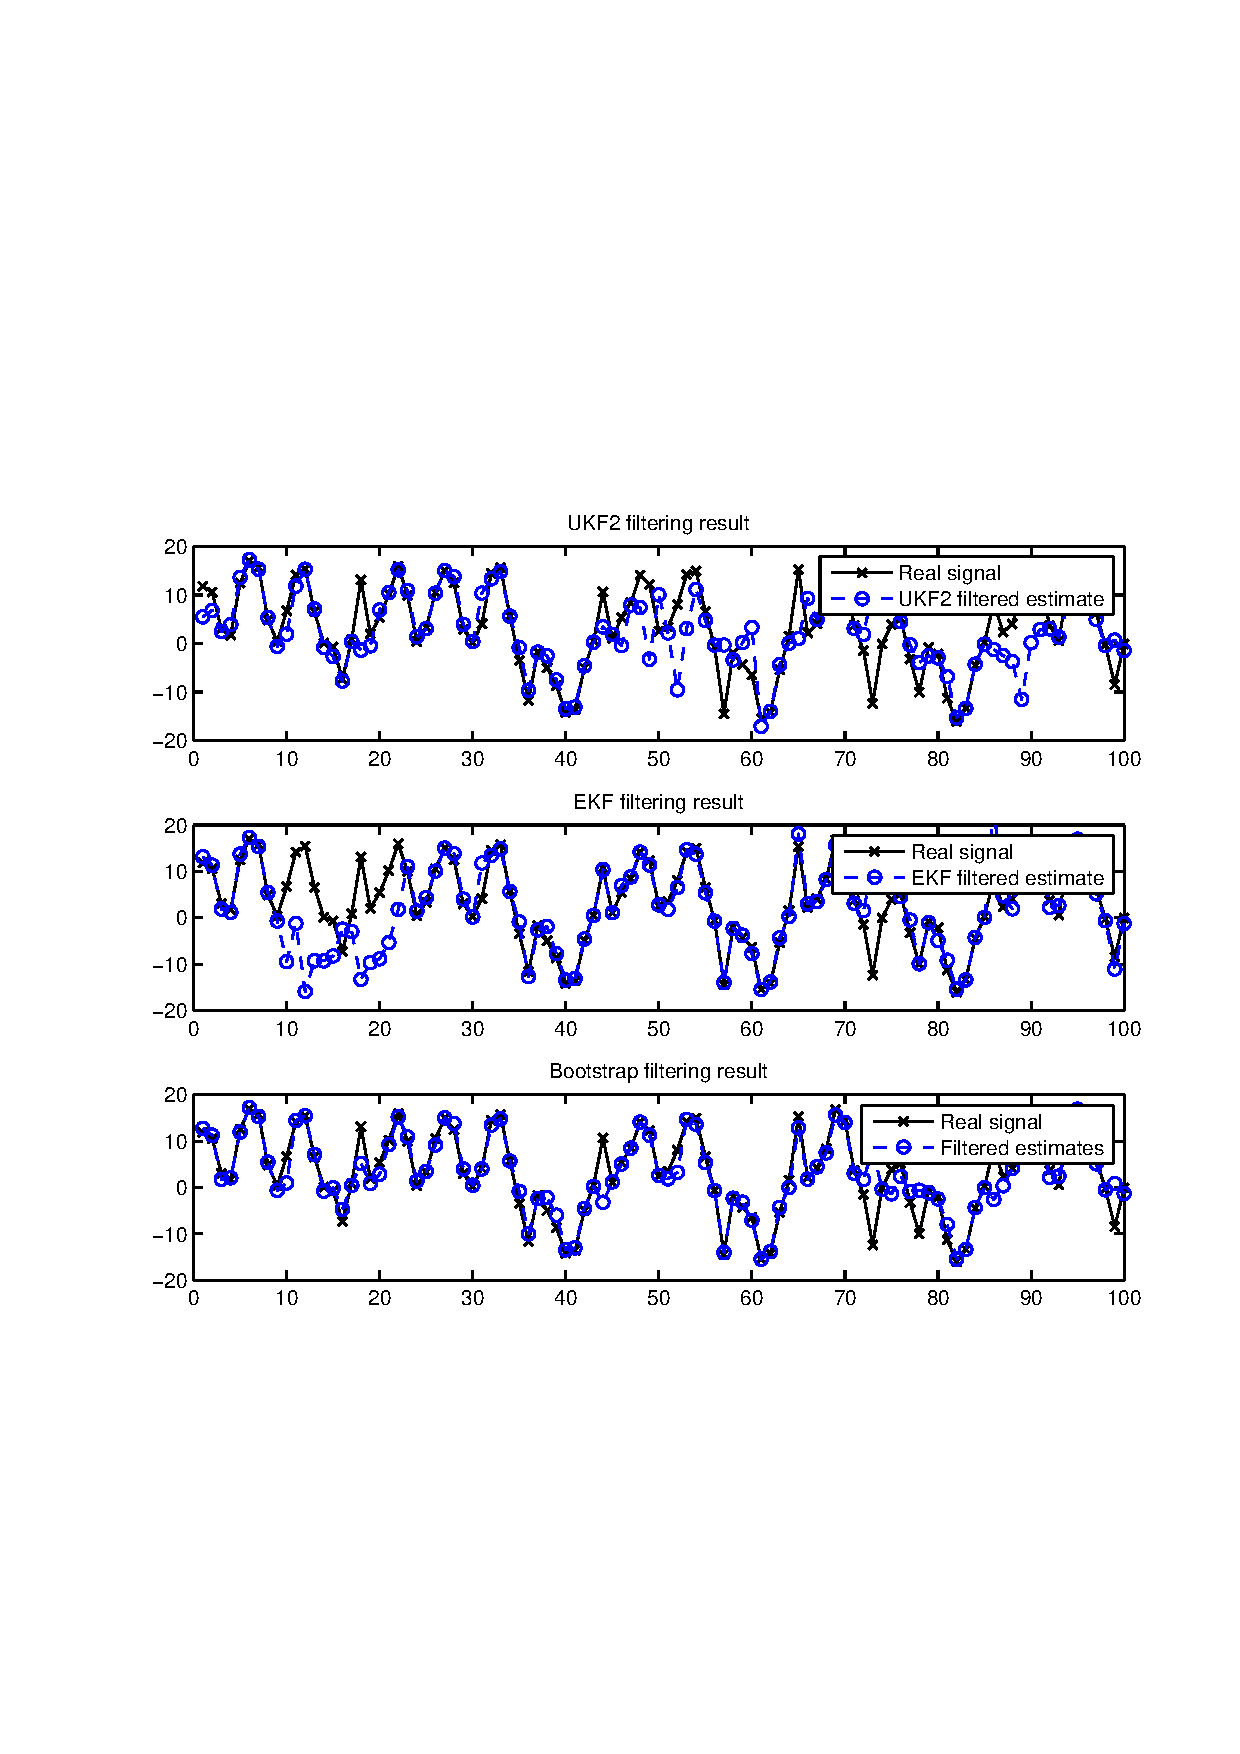
\includegraphics[width=11cm]{pics/ungm_states}
\caption{First 100 samples of filtering results of EKF, augmented form
UKF and bootstrap filter for UNGM-model.}
\label{fig:ungm_states}
\end{center}
\end{figure}

In figure \ref{fig:ungm_c_errors} we have plotted the absolute errors
and $3\sigma$ confidence intervals of the previous figures filtering
results. It can be seen that the EKF is overoptimistic in many cases
while UKF and boostrap filter are better at telling when their results
are unreliable. Also the lower error of bootstrap filter can be seen
from the figure. The bimodality is also easy to notice on those
samples, which were mentioned above.

\begin{figure}
\begin{center}
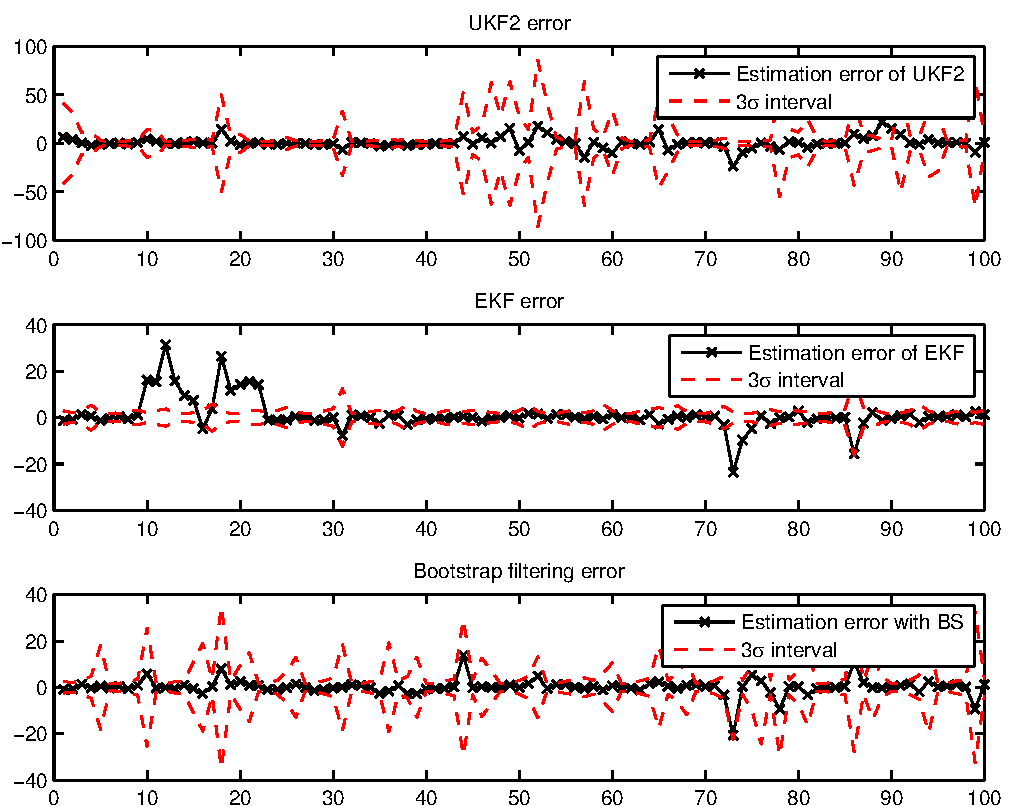
\includegraphics[width=11cm]{pics/ungm_c_errors}
\caption{Absolute errors of and $3\sigma$ confidence intervals of EKF,
augmented form UKF and bootstrap in 100 first samples.}
\label{fig:ungm_c_errors}
\end{center}
\end{figure}

The make a comparison between nonaugmented and augmented UKF we have
plotted 100 first samples of their filtering results in figure
\ref{fig:ungm_ukf_comp}. Results are very surprising (although same as
in \citet{Wu+Hu+Wu+Hu:2005}). The reason why nonaugmented UKF gave so bad
results is not clear. However, the better performance of augmented
form UKF can be explained by the fact, that the process noise is taken
into account more effectively when the sigma points are propagated
through nonlinearity. In this case it seems to be very crucial, as the
model is highly nonlinear and multi-modal.

\begin{figure}
\begin{center}
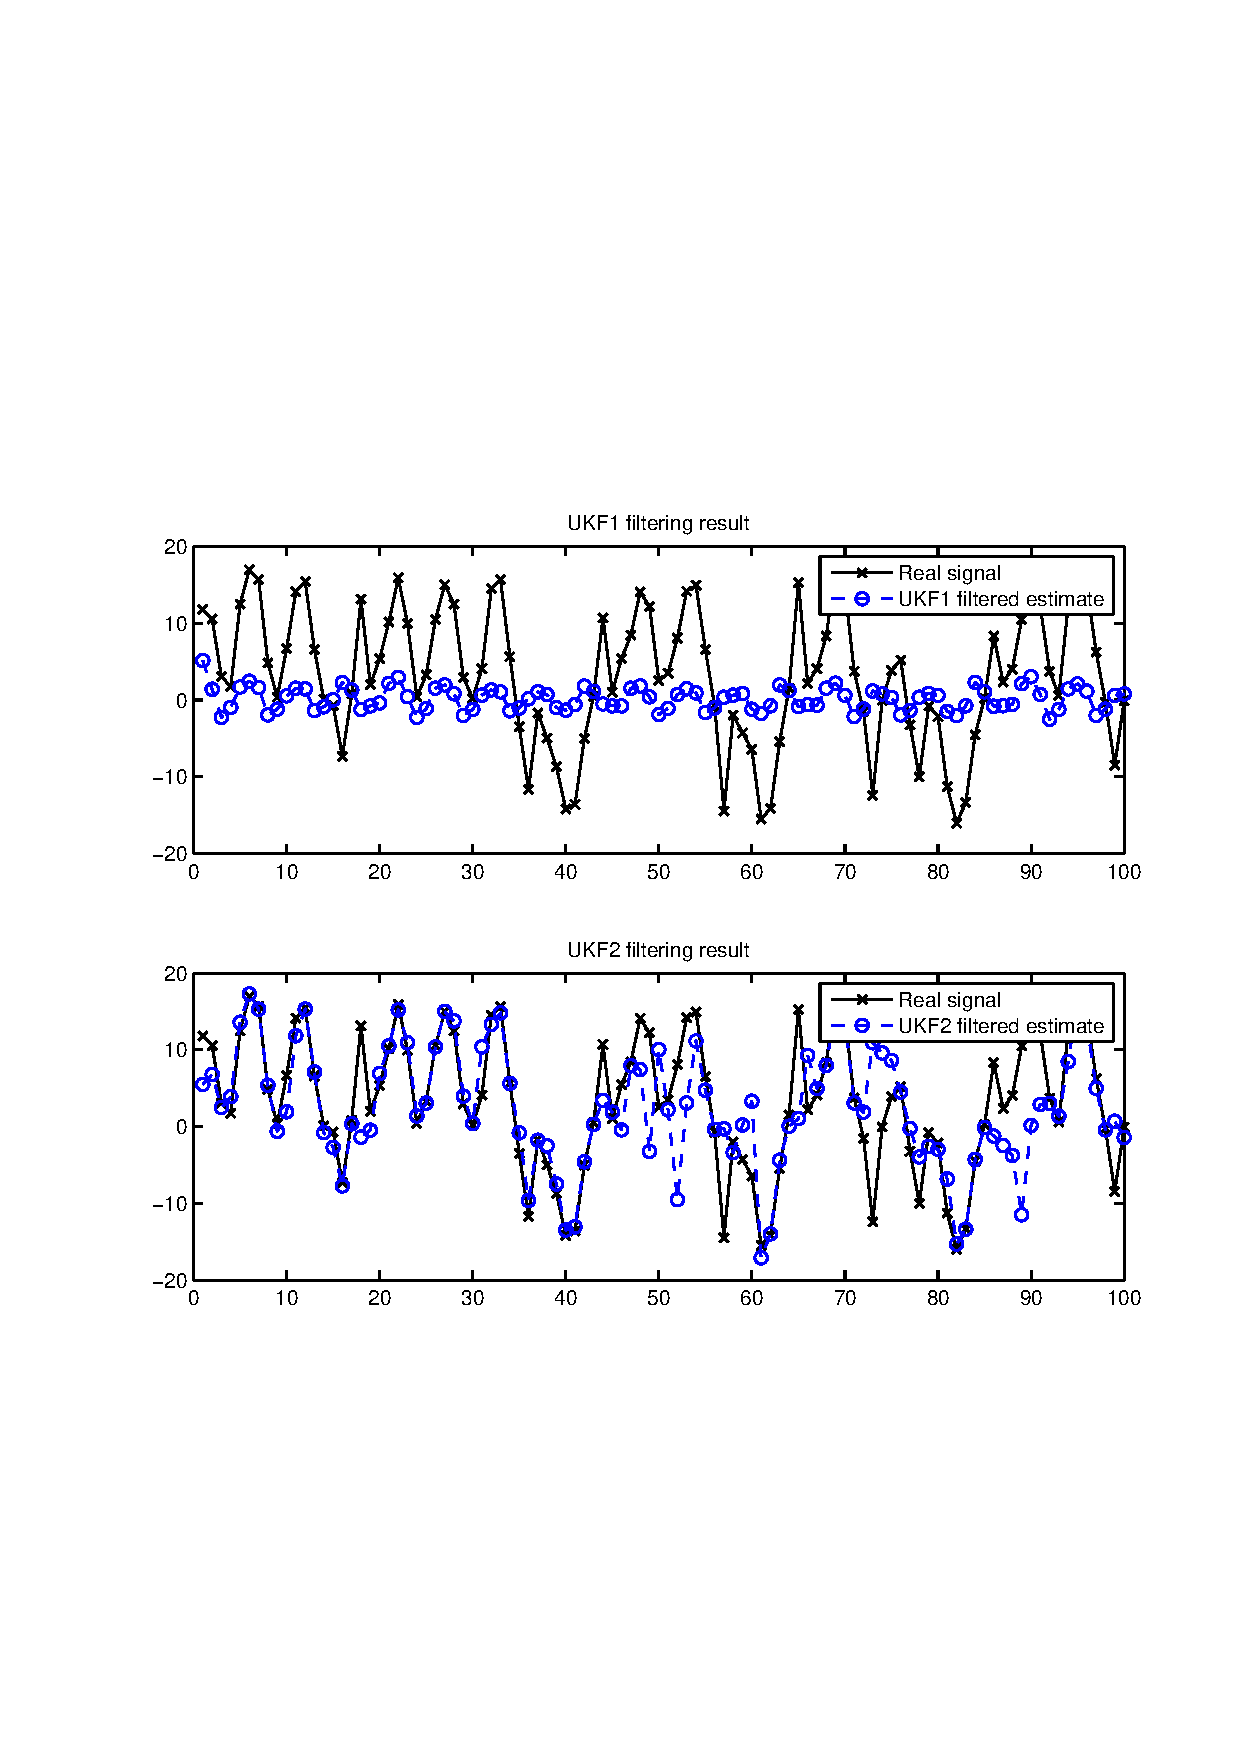
\includegraphics[width=11cm]{pics/ungm_ukf_comp}
\caption{Filtering results of nonaugmented UKF (UKF1) and augmented
UKF (UKF2) of 100 first samples.}
\label{fig:ungm_ukf_comp}
\end{center}
\end{figure}

Lastly in figure \ref{fig:ungm_mse} we have plotted the mean square
errors of each tested methods of 100 Monte Carlo runs. Average of
those errors are listed in table \ref{table:ungm_errors}. Here is a
discussion for the results:
%
\begin{itemize}
\item It is surprising that the nonaugmented UKF seems to be better
than EKF, while in above figures we have shown, that the nonaugmented
UKF gives very bad results. Reason for this is simple: the variance of
the actual signal is approximately 100, which means that by simply
guessing zero we get better performance than with EKF, on average. The
estimates of nonaugmented UKF didn't variate much on average, so they
were better than those of EKF, which on the other hand variated
greatly and gave huge errors in some cases. Because of this neither of
the methods should be used for this problem, but if one has to choose
between the two, that would be EKF, because in some cases it still
gave (more or less) right answers, whereas UKF were practically always
wrong.
\item The second order EKF were also tested, but that diverged almost
instantly, so it were left out from comparison.
\item Augmented form UKF gave clearly the best performance from the
tested Kalman filters. As discussed above, this is most likely due to
the fact that the process noise terms are propagated through the
nonlinearity, and hence odd-order moment information is used to obtain
more accurate estimates. The usage of RTS smoother seemed to improve
the estimates in general, but oddly in some cases it made the
estimates worse. This is most likely due to the multi-modality of the
filtering problem.
\item The Gauss--Hermite method performed rather well in both filtering and
smoothing. This was mostly due to the degree of approximation as the
rule entailed 10 sigma points.
\item The cubature Kalman filter gave results close to the UKF variants,
which is to no surprise as the filter uses similar sigma points.
\item Bootstrap filtering solution was clearly superior over all other
tested methods. The results had been even better, if greater amount of
particles had been used.
\end{itemize}

The reason why Kalman filters didn't work that well in this case is
because Gaussian approximations do not in general apply well for
multi-modal cases. Thus, a particle filtering solution should be
preferred over Kalman filters in such cases. However, usually the
particle filters need a fairly large amount of particles to be
effective, so they are generally more demanding in terms of
computational power than Kalman filters, which can be a limiting
factor in real world applications. The errors, even with bootstrap
filter, were also relatively large, so one must be careful when using
the estimates in, for example, making financial decisions. In practice
this means that one has to monitor the filter's covariance estimate,
and trust the state estimates and predictions only when the covariance
estimates are low enough, but even then there is a change, that the
filter's estimate is completely wrong.


\begin{figure}
\begin{center}
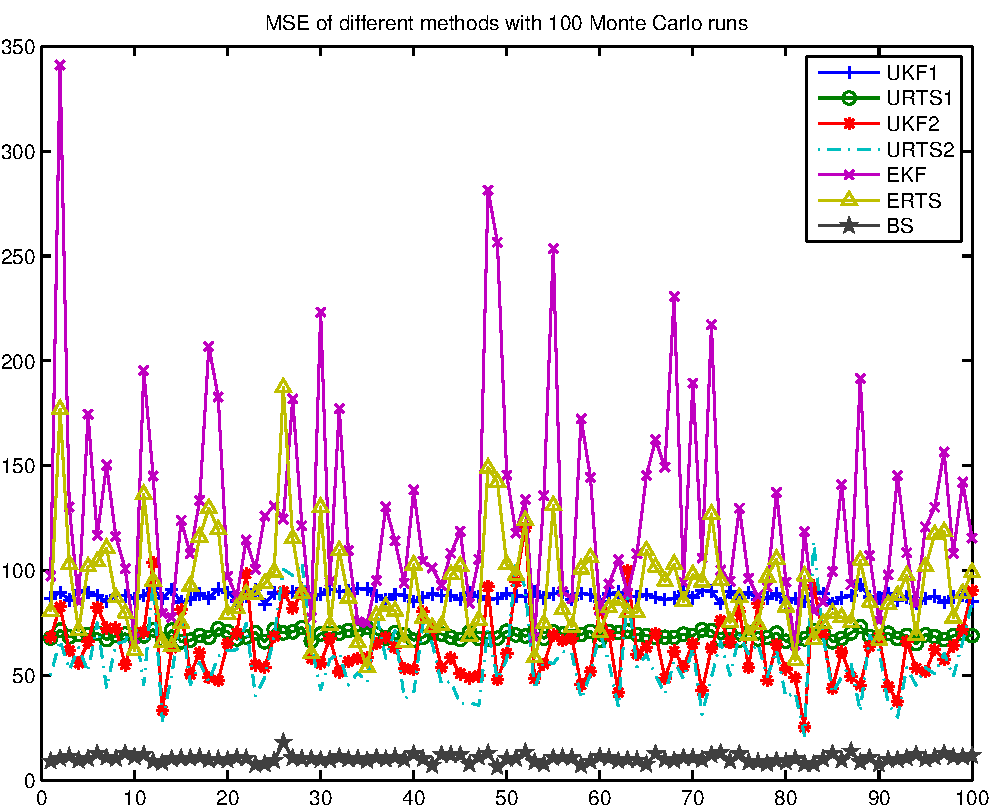
\includegraphics[width=11cm]{pics/ungm_mse}
\caption{MSEs of different methods in 100 Monte Carlo runs.}
\label{fig:ungm_mse}
\end{center}
\end{figure}

\begin{table}
\begin{center}
\begin{tabular}{|l|l|} \hline {\it Method}&{\it MSE[$x$]}\\ \hline
UKF1 & 87.9 \\ URTS1& 69.09 \\ UKF2 & 63.7 \\ URTS2 & 57.7 \\ EKF &
125.9 \\ ERTS & 92.2 \\ BS & 10.2 \\
GHKF & 40.9 \\
GHRTS & 31.6 \\
CKF & 72.3 \\
CRTS & 71.4 \\
 \hline
\end{tabular}
\caption{MSEs of estimating the UNGM model over 100 Monte Carlo
simulations.}
\label{table:ungm_errors}
\end{center}
\end{table}
 



\clearpage
\section{Demonstration: Bearings Only Tracking}

Next we review a classical filtering application \citep[see, e.g.,][]{Bar-Shalom+Li+Kirubarajan:2001}, in which we track a moving object with
sensors, which measure only the bearings (or angles) of the object
with respect positions of the sensors. There is a one moving target in
the scene and two angular sensors for tracking it. Solving this
problem is important, because often more general multiple target
tracking problems can be partitioned into sub-problems, in which
single targets are tracked separately at a time \citep{Sarkka+Vehtari+Lampinen:2007}.

The state of the target at time step $k$ consists of the position in
two dimensional cartesian coordinates $x_k$ and $y_k$ and the velocity
toward those coordinate axes, $\dot{x}_k$ and $\dot{y}_k$. Thus, the
state vector can be expressed as
%
\begin{equation}
%
\vec{x}_k =
\begin{pmatrix} x_k & y_k & \dot{x}_k & \dot{y}_k
\end{pmatrix}^T.
%
\end{equation}
%
The dynamics of the target is modelled as a linear, discretized Wiener
velocity model \citep{Bar-Shalom+Li+Kirubarajan:2001}
%
\begin{equation}
%
\vec{x}_k = \begin{pmatrix} 1 & 0 & \dt & 0 \\ 0 & 1 & 0 & \dt \\ 0 &
0 & 1 & 0 \\ 0 & 0 & 0 & 1
\end{pmatrix} % *
\begin{pmatrix} x_{k-1} \\ y_{k-1} \\ \dot{x}_{k-1} \\ \dot{y}_{k-1}
\end{pmatrix} + \vec{q}_{k-1},
%
\end{equation}
% 
where $\vec{q}_{k-1}$ is Gaussian process noise with zero mean and
covariance
%
\begin{equation}
\begin{split} E[\vec{q}_{k-1}\vec{q}^T_{k-1}] = \begin{pmatrix}
\frac{1}{3}\dt^3 & 0 & \frac{1}{2}\dt^2 & 0 \\ 0 & \frac{1}{3}\dt^3 &
0 & \frac{1}{2}\dt^2 \\ \frac{1}{2}\dt^2 & 0 & \dt & 0 \\ 0 &
\frac{1}{2}\dt^2 & 0 & \dt
\end{pmatrix} \\
\end{split}q,
\end{equation}
%
where $q$ is the spectral density of the noise, which is set to
$q=0.1$ in the simulations. The measurement model for sensor $i$ is
defined as
%
\begin{equation}
%
\theta^i_k = \arctan \left( \frac{y_k - s^i_y}{x_k - s^i_x}\right) +
r^i_k,
%
\end{equation}
%
where $(s^i_x,s^i_y)$ is the position of sensor $i$ and $r^i_k \sim
N(0,\sigma^2)$, with $\sigma = 0.05$ radians. In figure
\ref{fig:bot_measurements} we have plotted a one realization of
measurements in radians obtained from both sensors. The sensors are
placed to $(s^1_x,s^1_y) = (-1,-2)$ and $(s^2_x,s^2_y) = (1,1)$.
%
\begin{figure}
\begin{center}
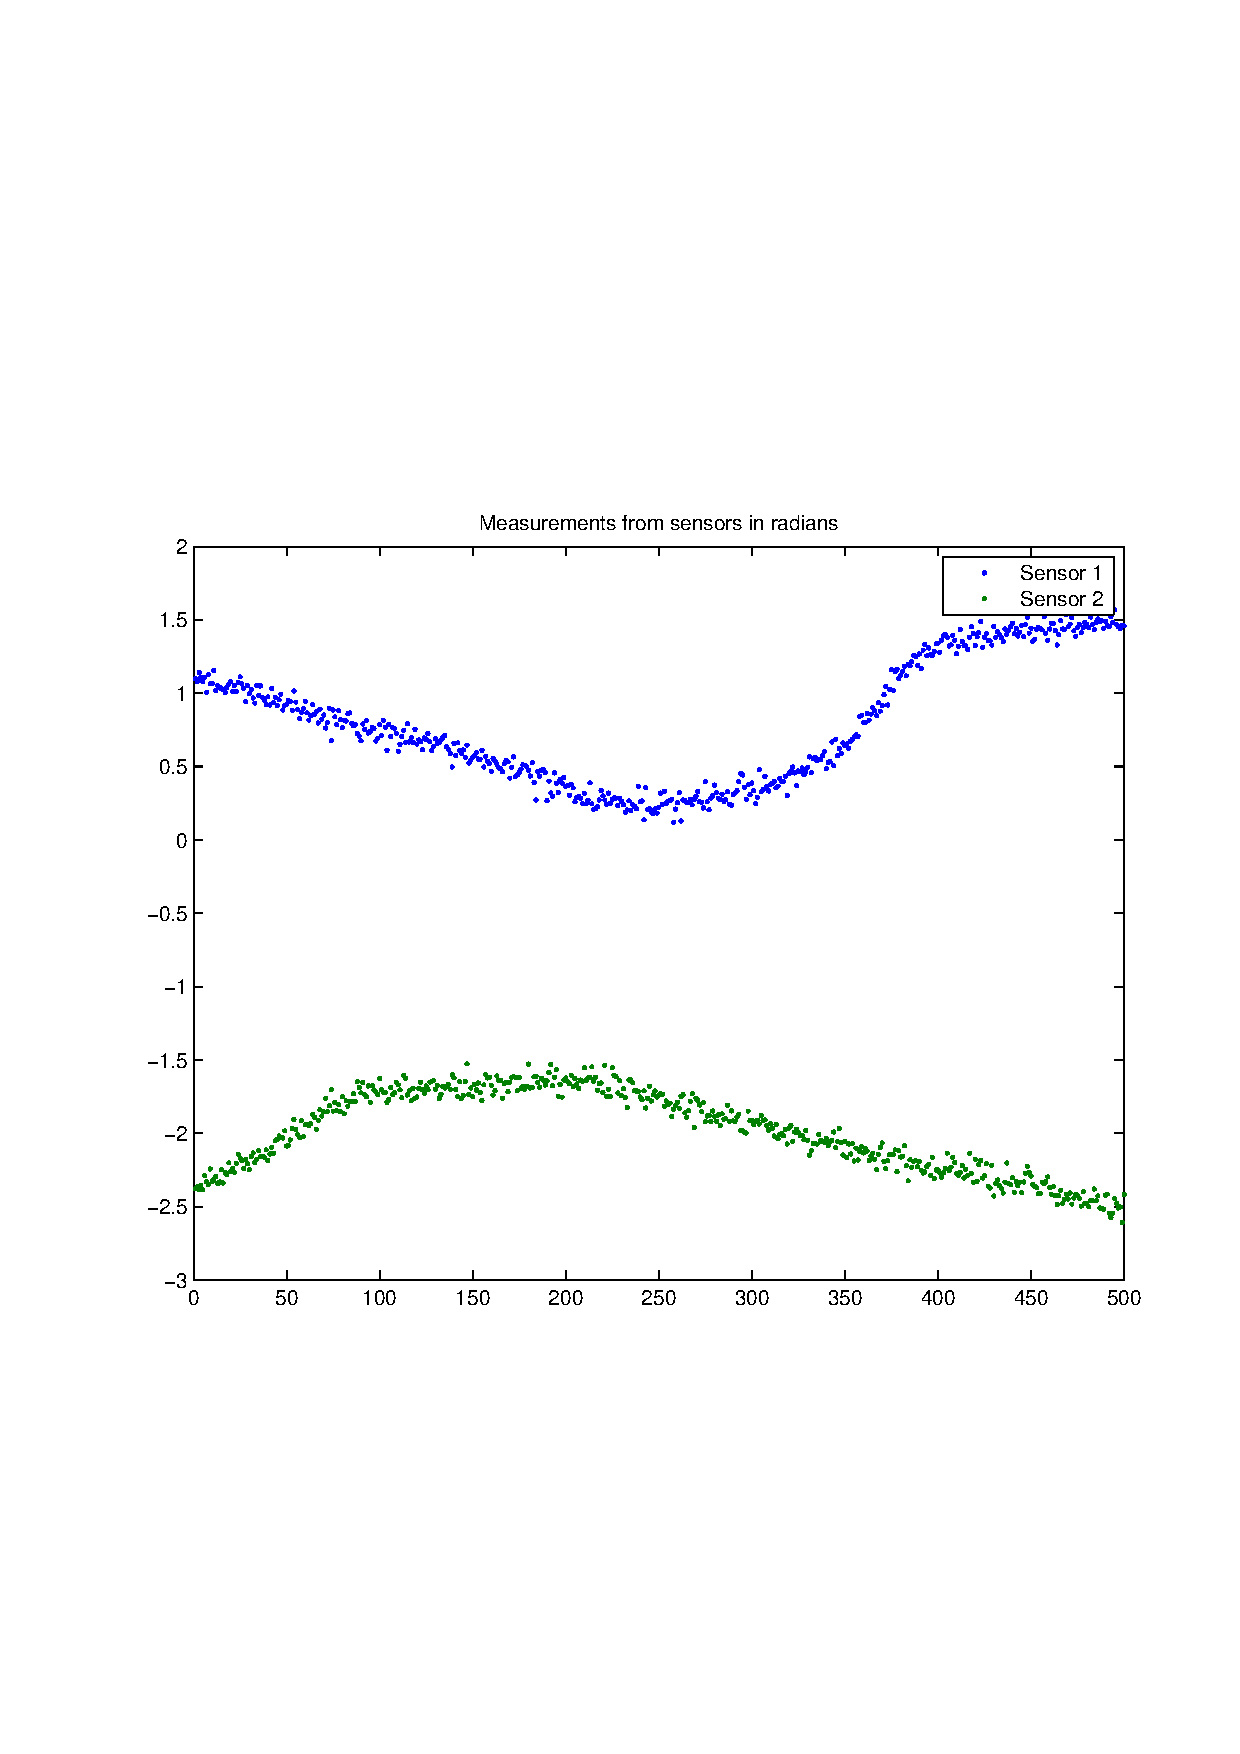
\includegraphics[width=11cm]{pics/bot_demo_measurements}
\caption{Measurements from sensors (in radians) in bearings only
tracking problem .}
\label{fig:bot_measurements}
\end{center}
\end{figure}

The derivatives of the measurement model, which are needed by EKF, can
be computed as
%
\begin{equation}
\begin{split} \frac{\partial \vec{h}^i(\vec{x}_k)}{\partial x_k} & =
\frac{-(y_k-s^i_y)}{(x_k-s^i_x)^2+(y_k-s^i_y)^2} \\ \frac{\partial
\vec{h}^i(\vec{x}_k)}{\partial y_k} & =
\frac{(x_k-s^i_x)}{(x_k-s^i_x)^2+(y_k-s^i_y)^2} \\ \frac{\partial
\vec{h}^i(\vec{x}_k)}{\partial \dot{x}_k} & = 0 \\ \frac{\partial
\vec{h}^i(\vec{x}_k)}{\partial \dot{y}_k} & = 0 , i = 1,2.
\end{split}
\label{eq:bot_dx}
\end{equation}
%
With these the Jacobian can written as
%
\begin{equation} \mat{H}_\vec{x}(\vec{x}_k,k) = \begin{pmatrix}
\frac{(x_k-s^1_x)}{(x_k-s^1_x)^2+(y_k-s^1_y)^2} &
\frac{-(y_k-s^1_y)}{(x_k-s^1_x)^2+(y_k-s^1_y)^2} & 0 & 0 \\
\frac{(x_k-s^2_x)}{(x_k-s^2_x)^2+(y_k-s^2_y)^2} &
\frac{-(y_k-s^2_y)}{(x_k-s^2_x)^2+(y_k-s^2_y)^2} & 0 & 0
\end{pmatrix}.
\end{equation}
%
The non-zero second order derivatives of the measurement function are
also relatively easy to compute in this model:
%
\begin{equation}
\begin{split} \frac{\partial^2 \vec{h}^i(\vec{x}_k)}{\partial x_k
\partial x_k} & =
\frac{-2(x_k-s^i_x)}{((x_k-s^i_x)^2+(y_k-s^i_y)^2)^2} \\
\frac{\partial^2 \vec{h}^i(\vec{x}_k)}{\partial x_k \partial y_k} & =
\frac{(y_k-s^i_y)^2-(x_k-s^i_x)^2}{((x_k-s^i_x)^2+(y_k-s^i_y)^2)^2} \\
\frac{\partial^2 \vec{h}^i(\vec{x}_k)}{\partial y_k \partial y_k} & =
\frac{-2(y_k-s^i_y)}{((x_k-s^i_x)^2+(y_k-s^i_y)^2)^2}.
\end{split}
\end{equation}
%
Thus, the Hessian matrices can be written as
%
\begin{equation} \mat{H}^i_\vec{xx}(\vec{x}_k,k) = \begin{pmatrix}
\frac{-2(x_k-s^i_x)}{((x_k-s^i_x)^2+(y_k-s^i_y)^2)^2} &
\frac{(y_k-s^i_y)^2-(x_k-s^i_x)^2}{((x_k-s^i_x)^2+(y_k-s^i_y)^2)^2} &
0 & 0 \\
\frac{(y_k-s^i_y)^2-(x_k-s^i_x)^2}{((x_k-s^i_x)^2+(y_k-s^i_y)^2)^2} &
\frac{-2(y_k-s^i_y)}{((x_k-s^i_x)^2+(y_k-s^i_y)^2)^2} & 0 & 0 \\ 0 & 0
& 0 & 0 \\ 0 & 0 & 0 & 0
\end{pmatrix}, i=1,2.
\end{equation}
%
We do not list the program code for the measurement function and it's
derivatives here as they are straightforward to implement, if the
previous examples have been read.

The target starts with state $\vec{x}_0 = \begin{pmatrix} 0 & 0 & 1 &
0
\end{pmatrix}$, and in the estimation we set the prior distribution
for the state to $\vec{x}_0 \sim N(\vec{0},\mat{P}_0)$, where
%
\begin{equation}
%
\mat{P}_0 = \begin{pmatrix} 0.1 & 0 & 0 & 0\\ 0 & 0.1 & 0 & 0\\ 0 & 0
& 10 & 0\\ 0 & 0 & 0 & 10
\end{pmatrix},
%
\end{equation}
%
which basically means that we are fairly certain about the target's
origin, but very uncertain about the velocity. In the simulations we
also give the target an slightly randomized acceleration, so that it
achieves a curved trajectory, which is approximately the same in
different simulations. The trajectory and estimates of it can be seen
in figures \ref{fig:bot_ekf1}, \ref{fig:bot_ekf2} and
\ref{fig:bot_ukf}. As can be seen from the figures EKF1 and UKF give
almost identical results while the estimates of EKF2 are clearly
worse. Especially in the beginning of the trajectory EKF2 has great
difficulties in getting on the right track, which is due to the
relatively big uncertainty in the starting velocity. After that the
estimates are fairly similar.

In table \ref{table:bot_rmse} we have listed the root mean square
errors (mean of position errors) of all tested methods (same as in
random sine signal example on page \pageref{page:sine_rmse} with the
addition of UTF) over 1000 Monte Carlo runs. The numbers prove the
previous observations, that the EKF1 and UKF give almost identical
performances. Same observations apply also to smoothers. Had the prior
distribution for the starting velocity been more accurate the
performance difference between EKF2 and other methods would have been
smaller, but still noticeable.

These observations also hold for the cubature methods. The Gauss--Hermite
Kalman filter and cubature Kalman filter give practically identical 
results as the unscented filter.

\begin{table}
\begin{center}
\begin{tabular}{|l|l|} \hline {\it Method}&{\it RMSE } \\ \hline 
  EKF1  & 0.114 \\ 
  ERTS1 & 0.054 \\ 
  ETF1  & 0.054 \\ 
  EKF2  & 0.202 \\ 
  ERTS2 & 0.074 \\ 
  ETF2  & 0.063 \\ 
  UKF   & 0.113 \\ 
  URTS  & 0.055 \\ 
  UTF   & 0.055 \\
  GHKF  & 0.107 \\
  GHRTS & 0.053 \\
  CKF   & 0.108 \\
  CRTS  & 0.053 \\
\hline
\end{tabular}
\caption{RMSEs of estimating the position in Bearings Only Tracking
problem over 1000 Monte Carlo runs. The Gauss--Hermite rule is of degree 3.}
\label{table:bot_rmse}
\end{center}
\end{table}

%
\begin{figure}
\begin{center}
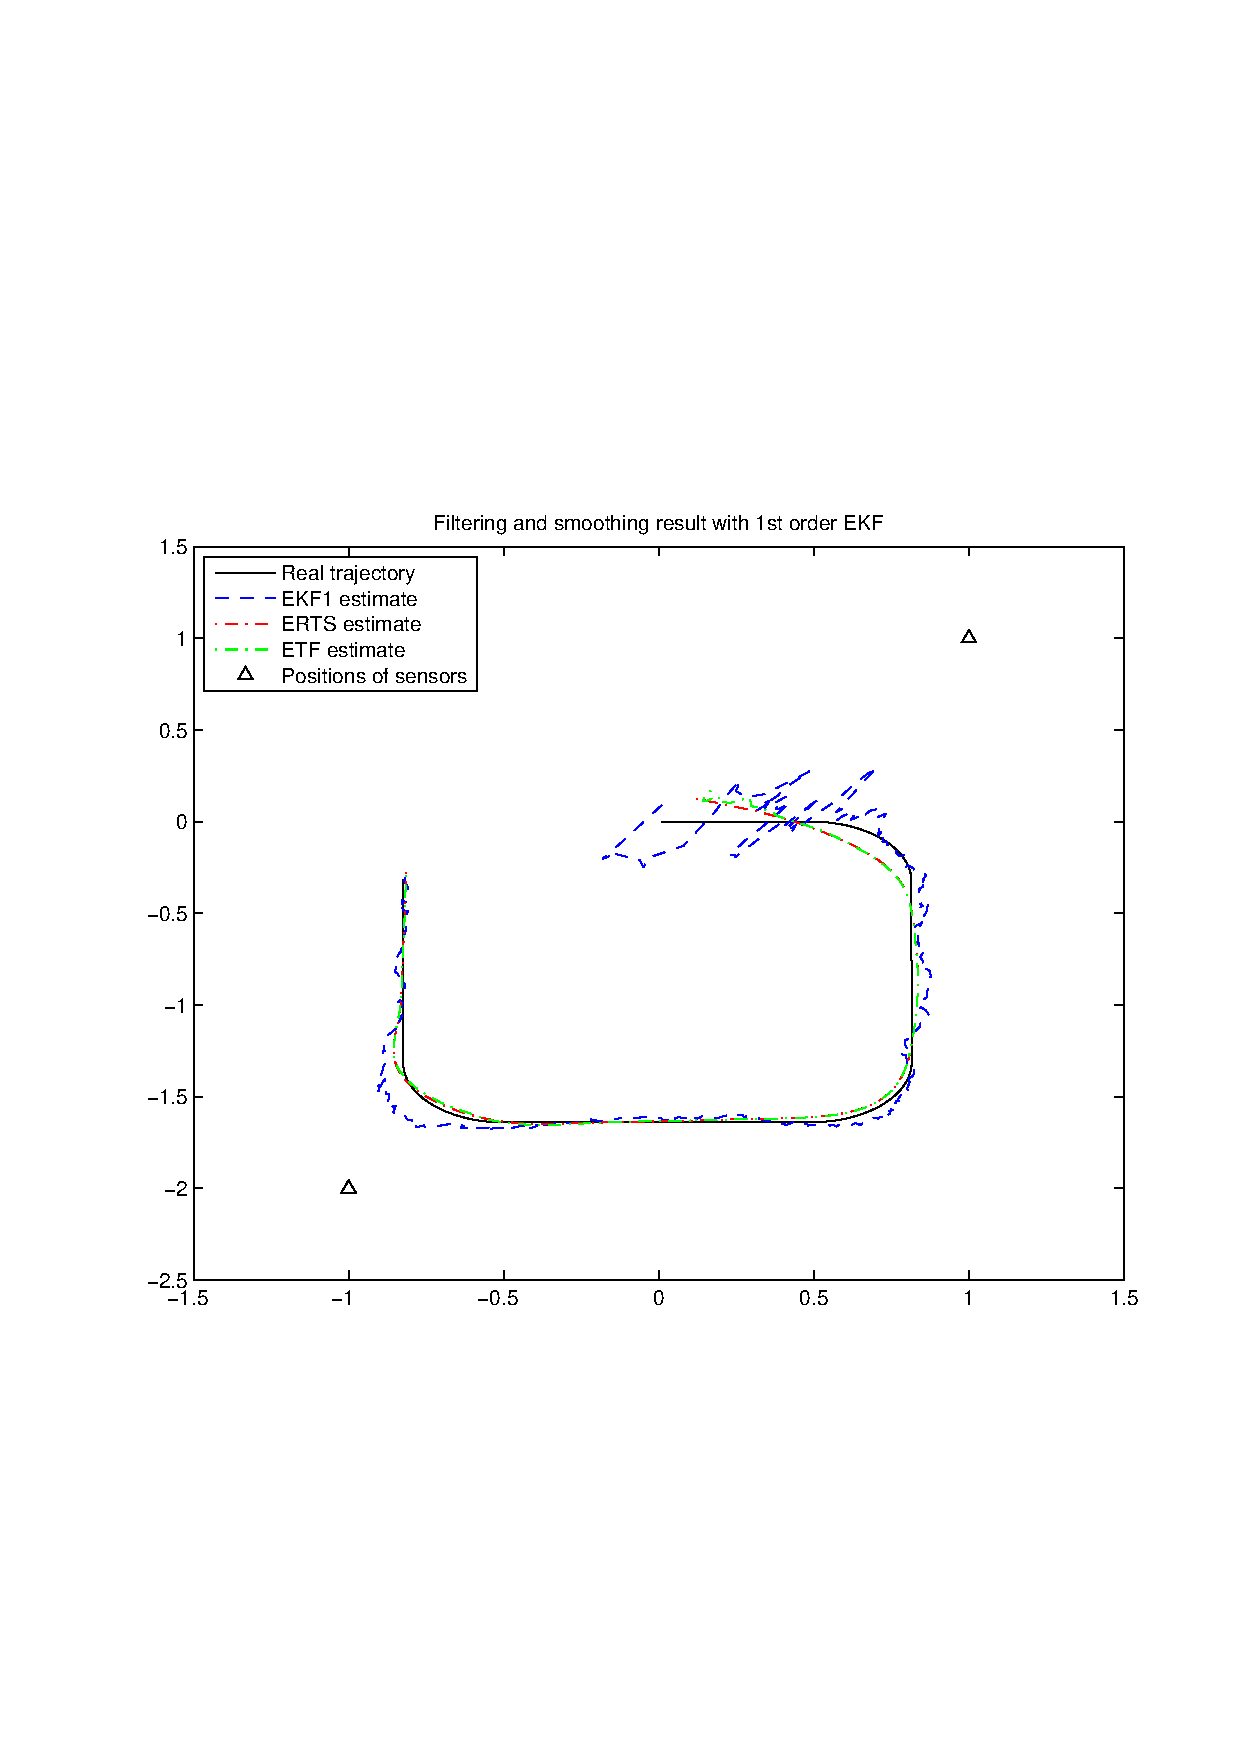
\includegraphics[width=11cm]{pics/bot_demo_ekf1}
\caption{Filtering and smoothing results of first order EKF.}
\label{fig:bot_ekf1}
\end{center}
\end{figure}

%
\begin{figure}
\begin{center}
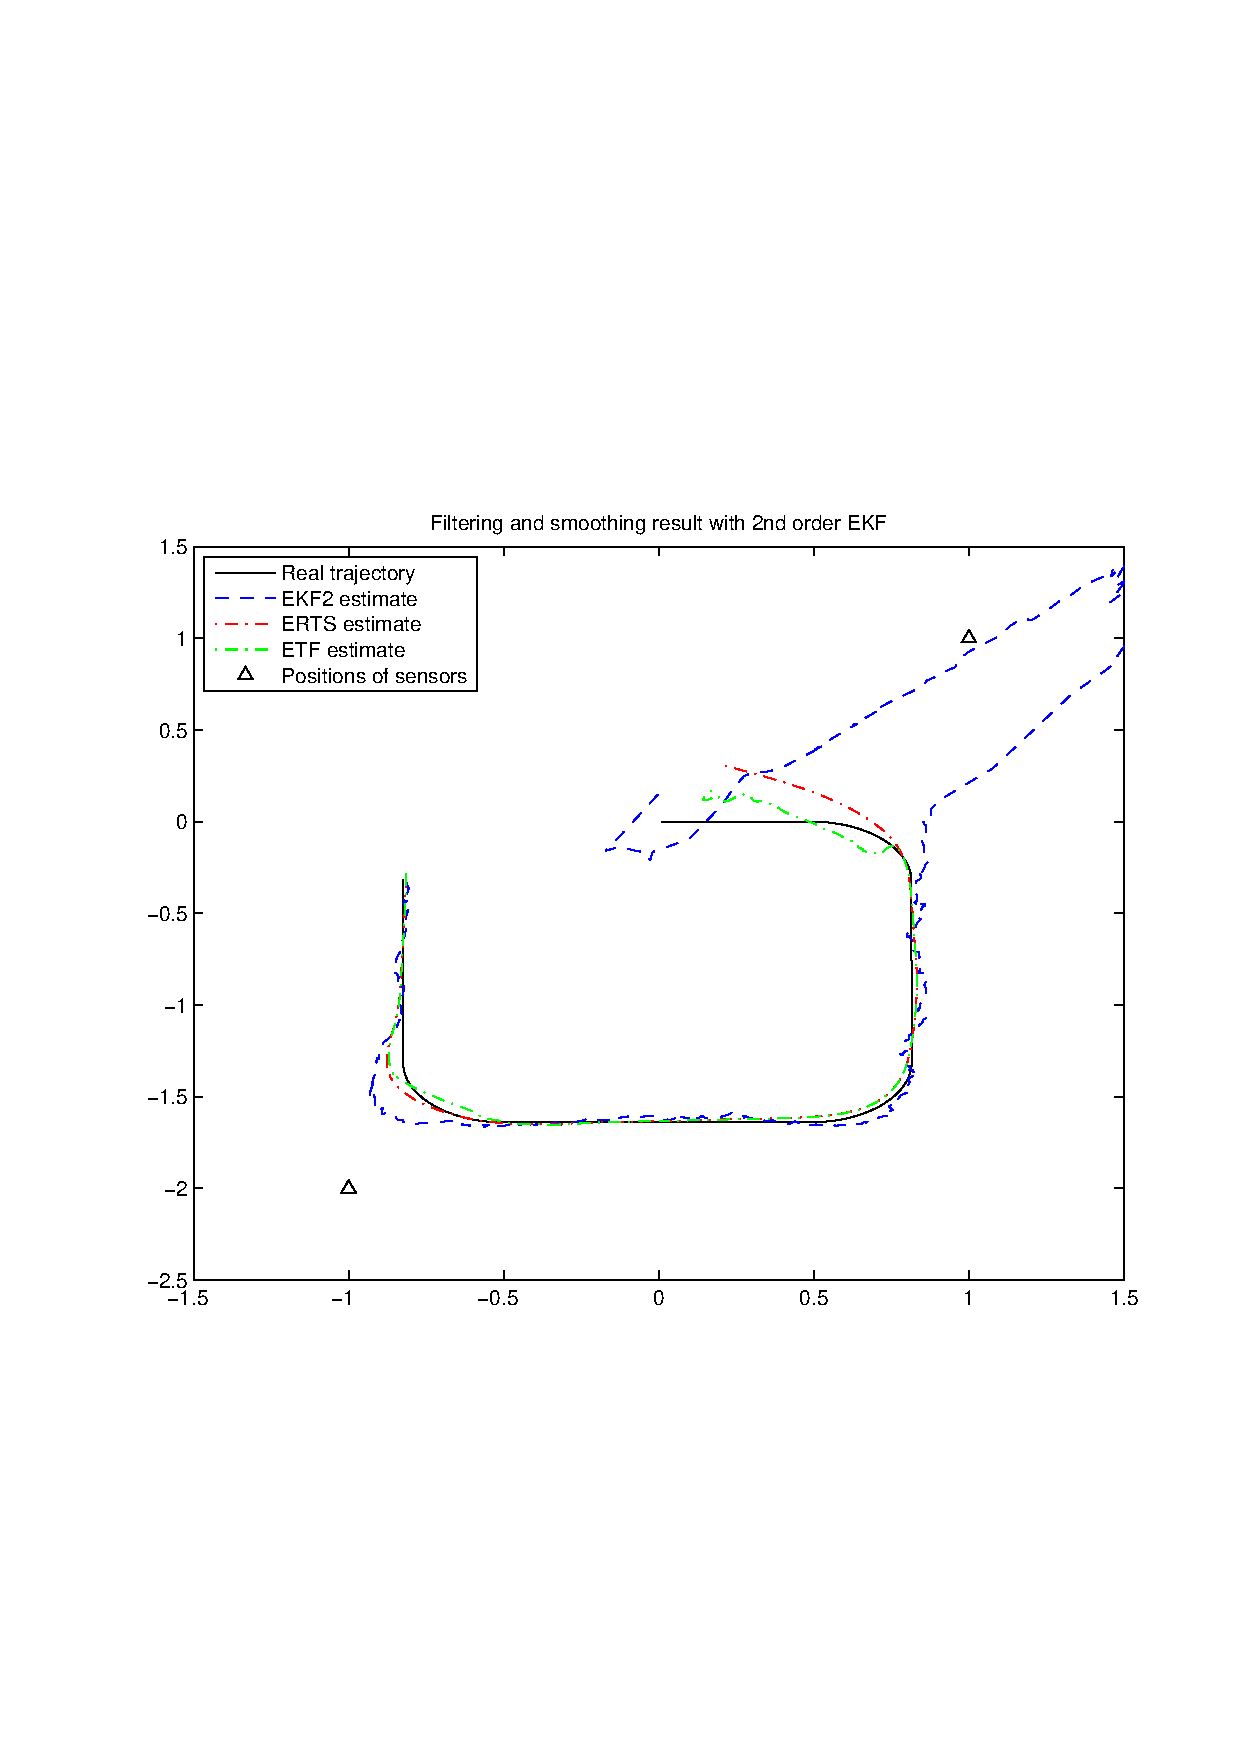
\includegraphics[width=11cm]{pics/bot_demo_ekf2}
\caption{Filtering and smoothing results of second order EKF.}
\label{fig:bot_ekf2}
\end{center}
\end{figure}

\begin{figure}
\begin{center}
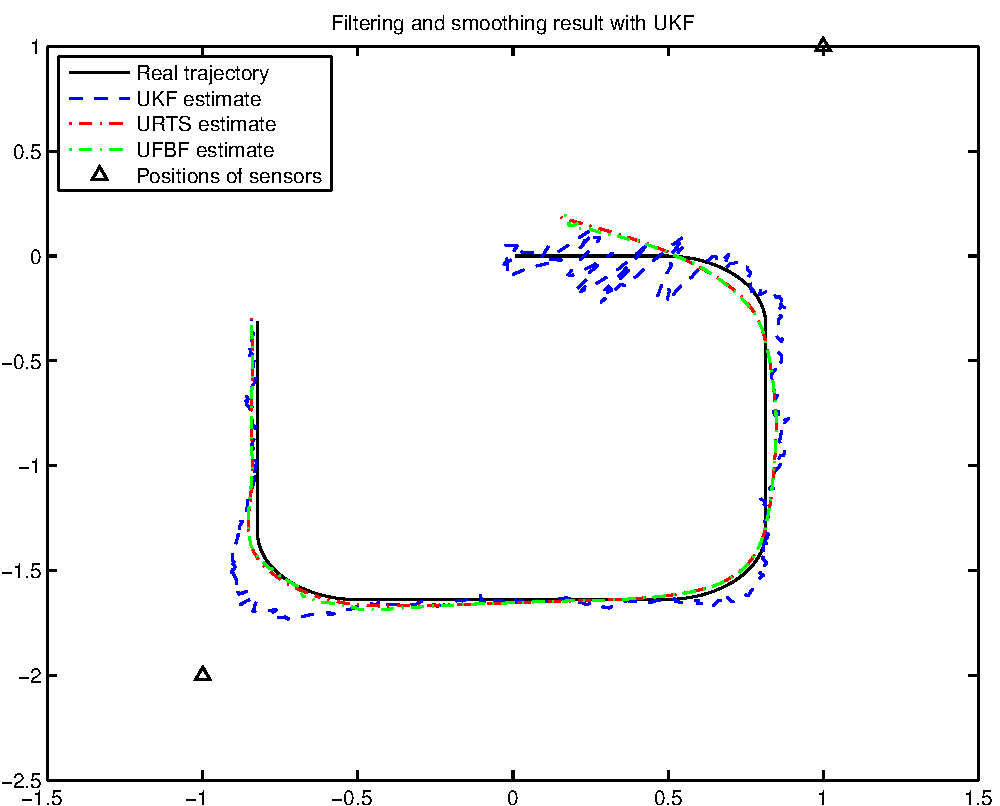
\includegraphics[width=11cm]{pics/bot_demo_ukf}
\caption{Filtering and smoothing results of UKF}
\label{fig:bot_ukf}
\end{center}
\end{figure}












\clearpage
\section{Demonstration: Reentry Vehicle Tracking}

Next we review a challenging filtering problem, which was used in
\citet{Julier+Uhlmann:2004} to demonstrate the performance of
UKF. Later they released few corrections to the model specifications
and simulation parameters in \citet{Julier+Uhlmann:2004b}.

This example conserns a reentry tracking problem, where radar is used
for tracking a space vehicle, which enters the atmosphere at high
altitude and very high speed. Figure \ref{fig:reentry_traj} shows a
sample trajectory of the vehicle with respect to earth and radar. The
dynamics of the vehicle are affected with three kinds of forces:
aerodynamic drag, which is a function of vehicle speed and has highly
nonlinear variations in altitude. The second type of force is gravity,
which causes the vehicle to accelerate toward the center of the
earth. The third type of forces are random buffeting terms. The state
space in this model consists of vehicles position ($x_1$ and $x_2$),
its velocity ($x_3$ and $x_4$) and a parameter of its aerodynamic
properties ($x_5$).  The dynamics in continuous case are defined as
\citep{Julier+Uhlmann:2004}
%
\begin{equation}
\begin{split}
%
\dot{x}_1(t) & = x_3(t) \\ \dot{x}_2(t) & = x_4(t) \\ \dot{x}_3(t) & =
D(t)x_3(t) + G(t)x_1(t) + v_1(t) \\ \dot{x}_4(t) & = D(t)x_4(t) +
G(t)x_2(t) + v_2(t) \\ \dot{x}_5(t) & = v_3(t),
%
\end{split}
\end{equation}
%
where $\vec{w}(t)$ is the process noise vector, $D(t)$ the
drag-related force and $G(t)$ the gravity-related force.  The force
terms are given by
%
\begin{equation}
\begin{split}
%
D(k) & = \beta(t) \exp \left\{ \frac{[R_0 - R(t)]}{H_0}\right\} V(t)
\\ G(t) & = -\frac{Gm_0}{R^3(t)} \\ \beta (t) & = \beta_0 \exp x_5(t),
%
\end{split}
\end{equation}
%
where $R(t) = \sqrt{x_1^2(t) + x_2^2(t)}$ is the vehicle's distance
from the center of the earth and $V(t) = \sqrt{x_3^2(t) + x_4^2(t)}$
is the speed of the vehicle.  The constants in previous definition
were set to
%
\begin{equation}
\begin{split}
%
\beta_0 & = -0.59783 \\ H_0 & = 13.406 \\ Gm_0 & = 3.9860 \times 10^5
\\ R_0 & = 6374.
%
\end{split}
\end{equation}
%
To keep the implementation simple the continuous-time dynamic
equations were discretized using a simple Euler integration scheme, to
give
%
\begin{equation}
\begin{split}
%
x_1(k+1) & = x_1(k) + \dt x_3(k) \\ x_2(k+1) & = x_2(k) + \dt x_4(k)
\\ x_3(k+1) & = x_3(k) + \dt (D(k)x_3(k) + G(k)x_1(k)) + w_1(k) \\
x_4(k+1) & = x_4(k) + \dt (D(k)x_4(k) + G(k)x_2(k)) + w_2(k) \\
x_5(k+1) & = x_5(k) + w_3(k),
%
\end{split}
\end{equation}
%
where the step size between time steps was set to $\dt = 0.1s$. Note
that this might be too simple approach in real world applications due
to high nonlinearities in the dynamics, so more advanced integration
scheme (such as Runge-Kutta) might be more preferable. The discrete
process noise covariance in the simulations was set to
%
\begin{equation}
%
Q(k) = \begin{pmatrix} 2.4064 \times 10^{-5} & 0 & 0 \\ 0 & 2.4064
\times 10^{-5} & 0 \\ 0 & 0 & 10^{-6}
\end{pmatrix}.
%
\end{equation}
%
The lower right element in the covariance was initially in \citet{Julier+Uhlmann:2004} set to zero, but later in \citet{Julier+Uhlmann:2004b}
changed to $10^{-6}$ to increase filter stability.


The non-zero derivatives of the discretized dynamic equations with
respect to state variables are straightforward (although rather
technical) to compute:
%
\begin{equation}
\begin{split}
%
\frac{\partial x_1(k+1)}{\partial x_1(k)} & = 1 \\ \frac{\partial
x_1(k+1)}{\partial x_3(k)} & = \dt \\ \frac{\partial
x_2(k+1)}{\partial x_2(k)} & = 1 \\ \frac{\partial x_2(k+1)}{\partial
x_4(k)} & = \dt \\
%
\frac{\partial x_3(k+1)}{\partial x_1(k)} & = \dt * (\frac{\partial
D(k)}{\partial x_1(k)} x_3(k) + \frac{\partial G(k)}{\partial x_1(k)}
x_1(k) + G(k)) \\ \frac{\partial x_3(k+1)}{\partial x_2(k)} & = \dt *
(\frac{\partial D(k)}{\partial x_2(k)} x_3(k) + \frac{\partial
G(k)}{\partial x_2(k)} x_1(k)) \\ \frac{\partial x_3(k+1)}{\partial
x_3(k)} & = \dt * (\frac{\partial D(k)}{\partial x_3(k)} x_3(k) +
D(k)) + 1 \\ \frac{\partial x_3(k+1)}{\partial x_4(k)} & = \dt *
(\frac{\partial D(k)}{\partial x_4(k)} x_3(k)) \\ \frac{\partial
x_3(k+1)}{\partial x_4(k)} & = \dt * (\frac{\partial D(k)}{\partial
x_5(k)} x_3(k)) \\
%
\frac{\partial x_4(k+1)}{\partial x_1(k)} & = \dt * (\frac{\partial
D(k)}{\partial x_1(k)} x_4(k) + \frac{\partial G(k)}{\partial x_1(k)}
x_2(k)) \\ \frac{\partial x_4(k+1)}{\partial x_2(k)} & = \dt *
(\frac{\partial D(k)}{\partial x_2(k)} x_4(k) + \frac{\partial
G(k)}{\partial x_2(k)} x_2(k) + G(k)) \\ \frac{\partial
x_4(k+1)}{\partial x_3(k)} & = \dt * (\frac{\partial D(k)}{\partial
x_3(k)} x_4(k)) \\ \frac{\partial x_4(k+1)}{\partial x_4(k)} & = \dt *
(\frac{\partial D(k)}{\partial x_4(k)} x_4(k) + D(k)) + 1 \\
\frac{\partial x_4(k+1)}{\partial x_5(k)} & = \dt * (\frac{\partial
D(k)}{\partial x_5(k)} x_4(k)) \\ \frac{\partial x_5(k+1)}{\partial
x_5(k)} & = 1,
%
\end{split}
\end{equation}
%
where the (non-zero) derivatives of the force, position and velocity
related terms with respect to state variables can be computed as
%
\begin{equation}
\begin{split}
%
\frac{\partial R(k)}{\partial x_1(k)} & = x_1(k) \frac{1}{R(k)} \\
\frac{\partial R(k)}{\partial x_2(k)} & = x_2(k) \frac{1}{R(k)} \\
\frac{\partial V(k)}{\partial x_3(k)} & = x_3(k) \frac{1}{V(k)} \\
\frac{\partial V(k)}{\partial x_4(k)} & = x_4(k) \frac{1}{V(k)} \\
\frac{\partial \beta(k)}{\partial x_5(k)} & = \beta(k)\frac{1}{R(k)}
\\ \frac{\partial D(k)}{\partial x_1(k)} & = -\frac{\partial
R(k)}{\partial x_1(k)} \frac{1}{H_0} * D(k) \\ \frac{\partial
D(k)}{\partial x_2(k)} & = -\frac{\partial R(k)}{\partial x_2(k)}
\frac{1}{H_0} * D(k) \\ \frac{\partial D(k)}{\partial x_3(k)} & =
\beta(k) \exp \left\{ \frac{[R_0 - R(k)]}{H_0}\right\} \frac{\partial
V(k)}{\partial x_3} \\ \frac{\partial D(k)}{\partial x_4(k)} & =
\beta(k) \exp \left\{ \frac{[R_0 - R(k)]}{H_0}\right\} \frac{\partial
V(k)}{\partial x_4} \\ \frac{\partial D(k)}{\partial x_5(k)} & =
\frac{\partial \beta(k)}{x_5(k)} \exp \left\{ \frac{[R_0 -
R(k)]}{H_0}\right\} V(k) \\ \frac{\partial G(k)}{\partial x_1(k)} & =
\frac{3 Gm_0}{(R(k))^4} \frac{\partial R(k)}{\partial x_1(k)} \\
\frac{\partial G(k)}{\partial x_2(k)} & = \frac{3 Gm_0}{(R(k))^4}
\frac{\partial R(k)}{\partial x_2(k)}.
%
\end{split}
\end{equation}
%
The prior distribution for the state was set to multivariate Gaussian,
with mean and covariance (same as in \citet{Julier+Uhlmann:2004})
%
\begin{equation}
\begin{split}
%
\vec{m}_0 & = \begin{pmatrix} 6500.4 \\ 349.14 \\ -1.8093 \\ -6.7967
\\ 0 \\
\end{pmatrix} \\ \mat{P}_0 & = \begin{pmatrix} 10^{-6} & 0 & 0 & 0 & 0
\\ 0 & 10^{-6}& 0 & 0 & 0 \\ 0 & 0 & 10^{-6} & 0 & 0 \\ 0 & 0 & 0 &
10^{-6}& 0 \\ 0 & 0 & 0 & 0 & 1
\end{pmatrix}.
%
\end{split}
\end{equation}
%
In the simulations the initial state were drawn from multivariate
Gaussian with mean and covariance
%
\begin{equation}
\begin{split}
%
\vec{m}_0 & = \begin{pmatrix} 6500.4 \\ 349.14 \\ -1.8093 \\ -6.7967
\\ 0.6932 \\
\end{pmatrix} \\ \mat{P}_0 & = \begin{pmatrix} 10^{-6} & 0 & 0 & 0 & 0
\\ 0 & 10^{-6}& 0 & 0 & 0 \\ 0 & 0 & 10^{-6} & 0 & 0 \\ 0 & 0 & 0 &
10^{-6}& 0 \\ 0 & 0 & 0 & 0 & 0
\end{pmatrix},
%
\end{split}
\end{equation}
%
that is, vehicle's aerodynamic properties were not known precisely
beforehand.

The radar, which is located at $(s_x, s_y) = (R_0,0)$, is used to
measure the range $r_k$ and bearing $\theta_k$ in relation to the
vehicle on time step $k$. Thus, the measurement model can be written
as
%
\begin{equation}
\begin{split}
%
r_k & = \sqrt{(x_1(k) - s_x)^2 + (x_2(k) - s_y)^2} + q_1(k) \\
\theta_k & = \tan^{-1} \left( \frac{x_2(k) - s_y}{x_1(k) - s_x}\right)
+q_2(k),
%
\end{split}
\end{equation}
%
where the measurement noise processes $q_1(k)$ and $q_2(k)$ are
Gaussians with zero means and standard deviations $\sigma_{r} =
10^{-3} \text{km}$ and $\sigma_{\theta} = 0.17 \text{mrad}$,
respectively. The derivatives of $\theta_k$ with respect to state
variables can computed with equations (\ref{eq:bot_dx}). For $r_k$ the
derivatives can be written as
%
\begin{equation}
\begin{split} \frac{\partial r_k}{\partial x_1(k)} & = x_1(k)
\frac{1}{r_k} \\ \frac{\partial r_k}{\partial x_2(k)} & = x_2(k)
\frac{1}{r_k}.
\end{split}
\end{equation}
%

\begin{figure}
\begin{center}
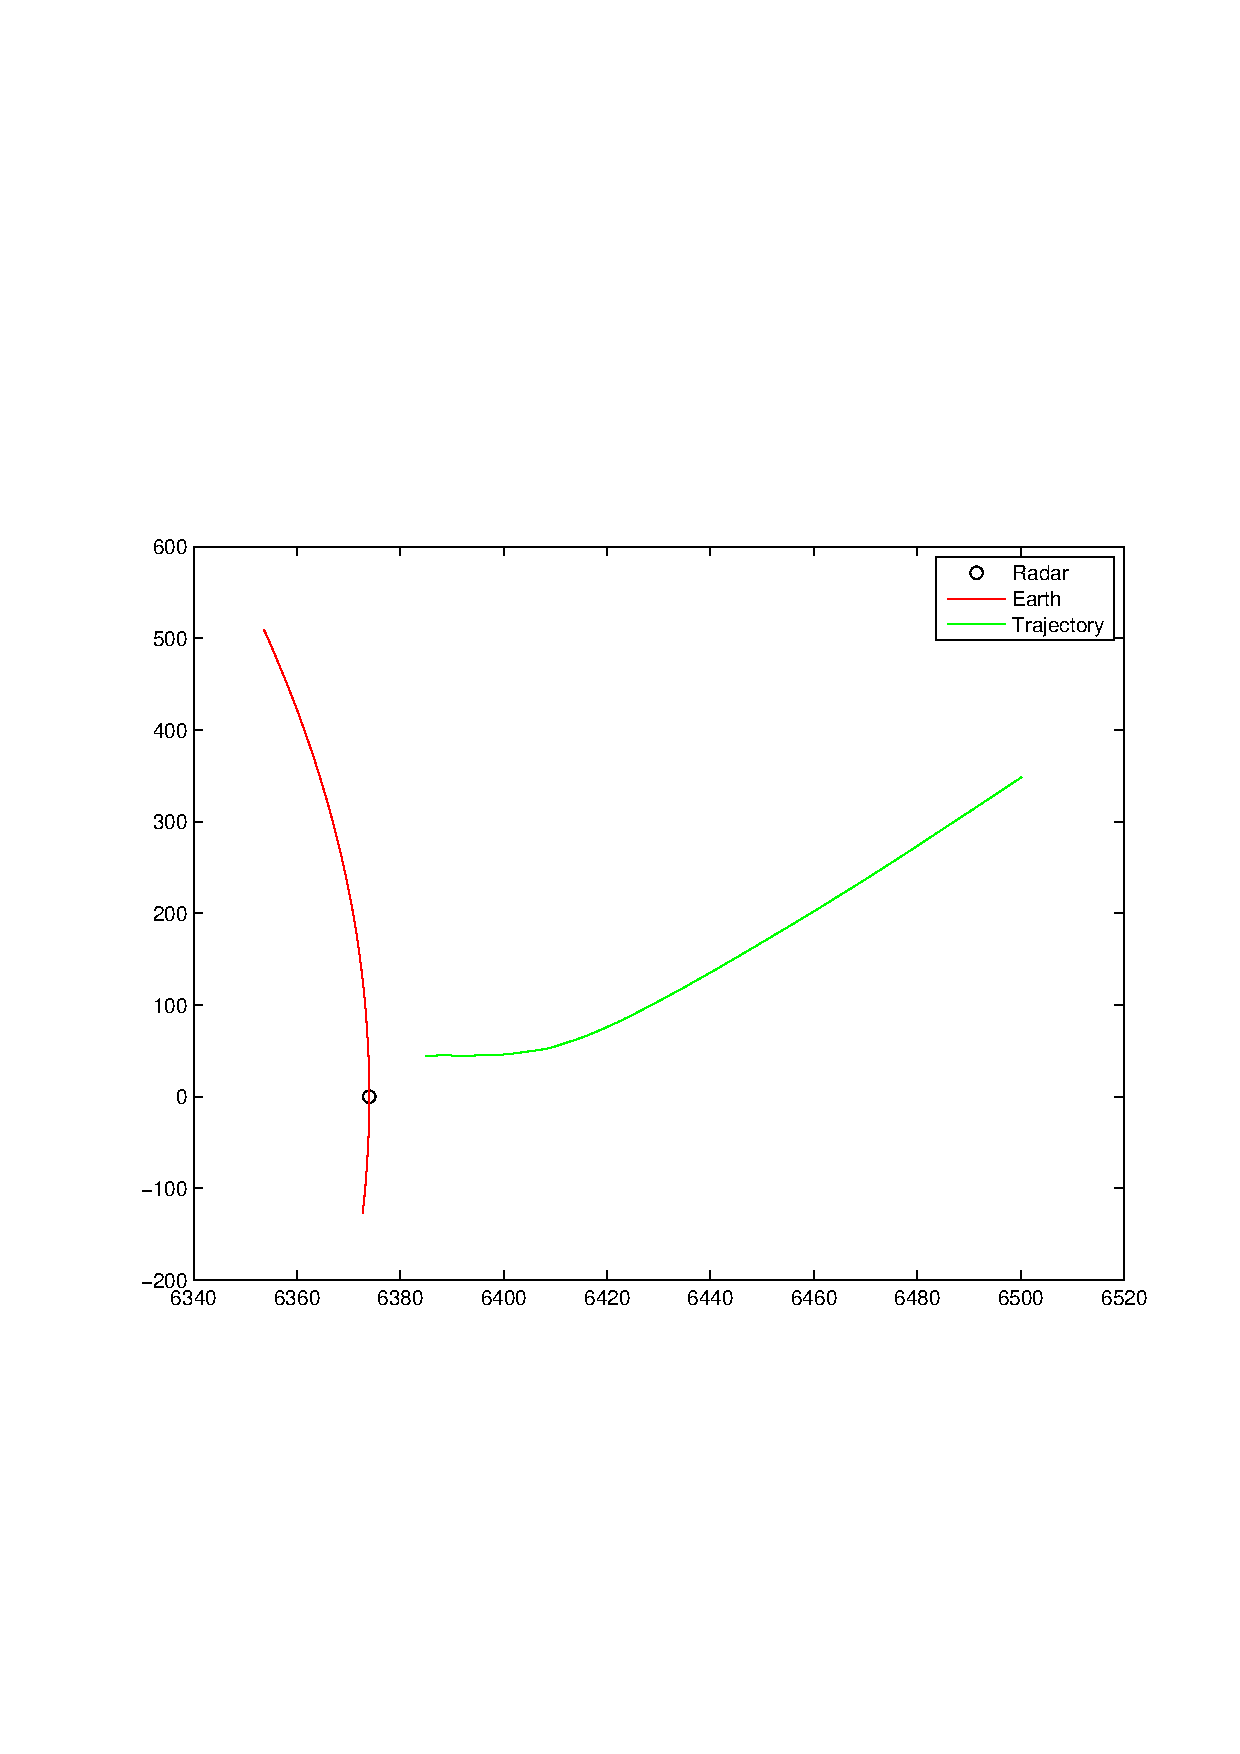
\includegraphics[width=11cm]{pics/reentry_trajectory}
\caption{Sample vehicle trajectory, earth and position of radar in
Reentry Vehicle Tracking problem.}
\label{fig:reentry_traj}
\end{center}
\end{figure}

In the table \ref{table:reentry_rmse} we have listed the RMS errors of
position estimates with tested methods, which were
%
\begin{itemize}
%
\item EKF1: first order extended Kalman filter.
\item ERTS: first order Rauch-Tung-Striebel smoother.
\item UKF: augmented form unscented Kalman filter.
\item URTS1: unscented Rauch-Tung-Striebel smoother with non-augmented
sigma points.
\item URTS2: unscented Rauch-Tung-Striebel smoother with augmented
sigma points.
\item UTF: unscented Forward-Backward smoother.
%
\end{itemize}
%
Extended Forward-Backward smoother was also tested, but it produced in
many cases divergent estimates, so it was left out from
comparison. Second order EKF was also left out, because evaluating the
Hessians would have taken too much work while considering the fact,
that the estimates might have gotten even worse.

From the error estimates we can see, that EKF and UKF --- and the
other methods as well --- give almost
identical performances, altough in the article \citep{Julier+Uhlmann:2004} UKF was clearly superior over EKF. The reason for this might be
the fact that they used numerical approximations (central differences)
for calculating the Jacobian in EKF rather than calculating the
derivatives in closed form, as was done in this demonstration.

In figure \ref{fig:reentry_errors} we have plotted the mean square
errors and variances in estimating $x_1$, $x_3$ and $x_5$ with EKF and
ERTS over 100 Monte Carlo runs. It shows that using smoother always
gives better estimates for positions and velocities, but for $x_5$ the
errors are practically the same after $\sim 45$ seconds. This also
shows that both methods are pessimistic in estimating $x_5$, because
variances were bigger than the true errors. Figures for $x_2$ and
$x_4$ are not shown, because they are very similar to the ones of
$x_1$ and $x_3$. Also by using UKF and URTS the resulting figures were
in practically identical, and therefore left out.
% 
%  
\begin{table}
\begin{center}
\begin{tabular}{|l|l|} \hline {\it Method}&{\it RMSE } \\ \hline
 EKF1  & 0.0084 \\ 
 ERTS  & 0.0044 \\ 
 UKF   & 0.0084 \\ 
 URTS1 & 0.0044 \\ 
 URTS2 & 0.0044 \\ 
 UTF   & 0.0044 \\
 GHKF  & 0.0084 \\
 GHRTS & 0.0049 \\
 CKF   & 0.0084 \\
 CRTS  & 0.0049 \\
 \hline
\end{tabular}
\caption{Average RMSEs of estimating the position in Reentry Vehicle
Tracking problem over 100 Monte Carlo runs. The Gauss--Hermite rule is
of degree 3.}
\label{table:reentry_rmse}
\end{center}
\end{table}
%
\begin{figure}
\begin{center}
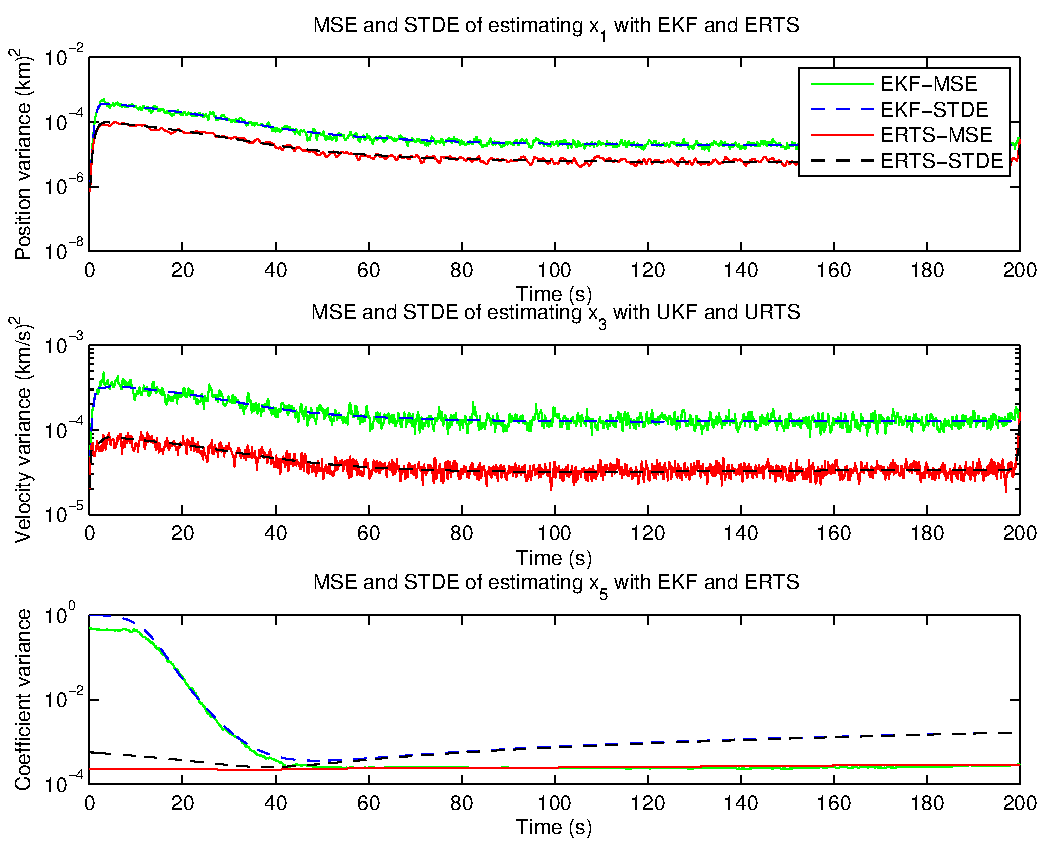
\includegraphics[width=11cm]{pics/reentry_errors}
\caption{MSEs and variances in estimating of $x_1$, $x_3$ and $x_5$
using EKF and ERTS over 100 Monte Carlo runs.}
\label{fig:reentry_errors}
\end{center}
\end{figure}


